\documentclass[11pt]{article}

% ==== PAGE GEOMETRY (matches QF journal: 160mm x 230mm type area) ====
\usepackage[
  textwidth=160mm, textheight=230mm,
  top=32mm, headheight=5pt, headsep=19pt, footskip=32pt
]{geometry}

% ==== FONTS (Times Roman, matching QF style) ====
\usepackage[T1]{fontenc}
\usepackage{mathptmx}

% ==== MATH ====
\usepackage{amsmath,amssymb,amsthm}

% ==== BIBLIOGRAPHY ====
\usepackage[round,authoryear]{natbib}

% ==== TABLES & FIGURES ====
\usepackage{graphicx,booktabs,rotating,multirow,tabularx}

% ==== LISTS ====
\usepackage{enumerate}

% ==== SECTION HEADINGS (QF style: bold, 11/13pt) ====
\usepackage{titlesec}
\titleformat{\section}
  {\fontsize{11}{13}\selectfont\bfseries\raggedright}{\thesection.}{0.5em}{}
\titleformat{\subsection}
  {\fontsize{11}{13}\selectfont\bfseries\itshape\raggedright}{\thesubsection.}{0.5em}{}
\titlespacing*{\section}{0pt}{26pt plus 4pt minus 2pt}{13pt}
\titlespacing*{\subsection}{0pt}{24pt plus 3pt minus 2pt}{7pt}

% ==== TYPOGRAPHY ====
\setlength{\parindent}{10pt}
\setlength{\parskip}{0pt}

% ==== TITLE (18/22pt bold uppercase, centred, like QF) ====
\makeatletter
\renewcommand{\maketitle}{%
  \clearpage\null
  \vspace*{42pt}%
  \begin{center}
    {\fontsize{18}{22}\selectfont\bfseries\MakeUppercase{\@title}\par}%
    \ifx\@author\@empty\else
      \vskip 21pt
      {\fontsize{13}{15}\selectfont\@author\par}%
    \fi
  \end{center}
  \vskip 18pt
}
\makeatother

% ==== ABSTRACT (9/11pt, indented 2pc both sides) ====
\renewenvironment{abstract}{%
  \fontsize{9}{11}\selectfont
  \setlength{\leftskip}{2pc}%
  \setlength{\rightskip}{2pc}%
  \noindent\ignorespaces
}{%
  \par\addvspace{32pt}%
}

% ==== KEYWORDS (9/11pt, indented, italic label) ====
\newenvironment{keywords}{%
  \par\addvspace{11pt}%
  \fontsize{9}{11}\selectfont
  \setlength{\leftskip}{2pc}%
  \setlength{\rightskip}{2pc plus 1fill}%
  \noindent{\itshape Keywords\/}: \ignorespaces
}{%
  \par\addvspace{26pt plus 4pt}%
}

% ==== JEL CLASSIFICATION (same style as keywords) ====
\newenvironment{classcode}{%
  \par\addvspace{-9pt}%
  \fontsize{9}{11}\selectfont
  \setlength{\leftskip}{2pc}%
  \setlength{\rightskip}{2pc plus 1fill}%
  \noindent{\itshape JEL Classification\/}: \ignorespaces
}{%
  \par\addvspace{26pt plus 4pt}%
}

% ==== HYPERLINKS ====
\usepackage[colorlinks=true,linkcolor=blue,citecolor=blue,urlcolor=blue]{hyperref}

% ==== APPENDICES (renames sections to "Appendix A: ...") ====
\newcommand{\appendices}{%
  \appendix
  \titleformat{\section}
    {\fontsize{11}{13}\selectfont\bfseries\raggedright}
    {Appendix \thesection:}{0.5em}{}%
}

% ==== CUSTOM COMMANDS ====
\newcommand{\proofref}[1]{%
  \par\noindent\hfill{\small\itshape\hyperref[#1]{$\triangleright$ Proof, p.\,\pageref{#1}}}}
\newcommand{\E}{\mathbb{E}}
\renewcommand{\P}{\mathbb{P}}
\newcommand{\R}{\mathbb{R}}
\newcommand{\diff}{\mathrm{d}}
\newcommand{\F}{\mathcal{F}}
\newcommand{\one}{\mathbf{1}}
\newcommand{\Rea}{\operatorname{Re}}

% ==== THEOREM ENVIRONMENTS ====
\theoremstyle{plain}
\newtheorem{theorem}{Theorem}[section]
\newtheorem{lemma}[theorem]{Lemma}
\newtheorem{proposition}[theorem]{Proposition}

\theoremstyle{definition}
\newtheorem{definition}{Definition}[section]
\newtheorem{assumption}{Assumption}[section]

\theoremstyle{remark}
\newtheorem{remark}{Remark}

\begin{document}

\title{Optimal Sizing of Leveraged Crypto Long--Short Positions under Kou Jump-Diffusion via Killed Moments}

\maketitle

\begin{abstract}
We study a leveraged crypto long--short position, held on a DeFi lending
protocol, whose solvency is governed by a collateral-to-liability health
factor and whose payoff is killed when that factor crosses a liquidation
boundary. Sizing such a position requires the survival probability and
killed-payoff moments at every candidate initial buffer. We derive a
semi-analytic Laplace-domain method for these quantities under bivariate Kou
double-exponential jump--diffusion dynamics. Compared with Monte Carlo
simulation, the method is free of sampling noise, stays accurate near the
liquidation boundary where discretely monitored simulation is least reliable,
and evaluates orders of magnitude faster, making repeated evaluation across
candidate buffers practical. We use these outputs to solve the initial-buffer
sizing problem under alternative liquidation constraints and moment-based
objectives, and a paired moving-block bootstrap shows that the selected buffer
is sensitive to calibration uncertainty.
\end{abstract}

\begin{keywords}
DeFi lending; crypto assets; leveraged long--short; killed payoff moments; health factor; Kou double-exponential jump diffusion; first-passage problem; Laplace resolvent
\end{keywords}

\begin{classcode}
G11; G12; C65
\end{classcode}

% ============================================================
\section{Introduction}
% ============================================================

Crypto-asset DeFi lending protocols such as AAVE and Compound enable a leveraged
long--short strategy: an investor deposits one crypto asset as collateral, borrows a
second crypto asset, and sells it short. The position is governed by a real-time
\emph{health factor}---a borrowing-power-adjusted ratio of collateral to liability---and
may be liquidated when that ratio falls below one. The resulting exposure combines
leveraged relative-value risk, a path-dependent liquidation boundary, discontinuous price
jumps, and state-dependent survival. Its initial health buffer controls both leverage and
distance to liquidation, but evaluating that trade-off first requires the distribution of a
payoff killed at the liquidation boundary.

The two recurring objects are the probability that the position survives to the horizon
and the moments of its killed terminal payoff, and both must be evaluated repeatedly across
candidate initial health buffers. Monte Carlo simulation can approximate them, but barrier
discretisation and sampling noise are especially consequential near liquidation, and
repeated simulation is costly inside a sizing search. The missing input for solving the
sizing problem is therefore not a universal economic objective, but a fast, repeatable map
from the initial buffer to survival probabilities and killed-payoff moments.

We work under a bivariate Kou double-exponential jump--diffusion model \citep{Kou2002} and
make four contributions. First, a unit-equity normalization collapses the two-asset
holding to a single initial health buffer, the natural sizing parameter, while liquidation
depends only on a one-dimensional log-price ratio between the two legs. Second, for each
admissible moment order, an exponential change of measure absorbs the short-leg price
factor, reducing the two-asset killed moment to a one-dimensional killed expectation of
that log-price ratio. Third, the double-exponential jump structure turns the resulting
Laplace-domain equation into algebra: in the generic case, three barrier conditions pin
down a fixed, low-dimensional linear system whose size does not grow with the moment
order; numerical Laplace inversion then recovers the time-domain quantities
\citep{Talbot1979}. Fourth, these objective-independent outputs turn initial-buffer sizing
into a one-dimensional optimization, which we illustrate under alternative liquidation
constraints and moment-based objectives without taking a position on which objective is
economically correct.

This paper sits at the intersection of the DeFi liquidation literature and the analytical
first-passage literature for jump diffusions. \citet{Qin2021} and
\citet{HeimbachHuang2024} document the incentive structure and leverage amplification of
DeFi liquidations, but do not provide the repeated killed-moment evaluation developed here.
\citet{KouWang2003} derive explicit Laplace-transform first-passage results under
double-exponential jump diffusion, and \citet{Sepp2004} extends this to barrier option
pricing; we instead price a barrier-killed long--short ratio, bridging the two settings via
the measure-change reduction above. More distantly, \citet{JacobsLevyStarer1999} advocate
joint optimisation of long and short legs, and \citet{DangForsyth2016} study dynamic
mean--variance control under jump risk; our sizing problem is a static analogue, optimizing
a single initial buffer against a killed-payoff distribution rather than a control process.

The scope of this framework is as follows. It evaluates liquidation
probabilities, killed payoff moments, and conditional surviving-path moments repeatedly
across initial health buffers, and solves the resulting sizing problem for a stated
objective.

The remainder of the paper is organised as follows. Section~\ref{sec:setup} defines the
position, the liquidation barrier, and the health-buffer parameterization.
Section~\ref{sec:model} specifies the bivariate Kou model and its tilted dynamics.
Section~\ref{sec:moments} reduces payoff moments to one-dimensional killed expectations,
and Section~\ref{sec:resolvent} derives their time-Laplace transforms and finite-dimensional
evaluation system. Section~\ref{sec:numerical} validates the numerical method, and
Section~\ref{sec:application} illustrates the initial-buffer sizing problem.
Section~\ref{sec:discussion} concludes. Appendix~\ref{sec:calibration} describes the
empirical calibration estimator, Appendix~\ref{app:downward-phases} derives the
downward-phase boundary conditions, and Appendix~\ref{app:proofs} collects the proofs.

% ============================================================
\section{Leveraged Long--Short Position and Health-Factor Barrier}\label{sec:setup}
% ============================================================

We consider a leveraged long--short portfolio in which an investor holds asset $S_1$
and owes asset $S_2$, with net initial equity normalized to one unit of account. The
position is liquidated if collateral becomes too small relative to the liability. This
section defines the barrier, the killed-payoff object studied in the paper, and the mapping
from the initial health buffer to holdings. No investor objective is needed for these
definitions.

\subsection{Health factor, liquidation time, and killed payoff}
Let $(\Omega,\F,(\F_t)_{t\ge 0},\P)$ be a filtered probability space.
Two strictly positive asset prices $S_1,S_2$ evolve as
\[
S_{i,t}=S_{i,0}e^{X_{i,t}},\qquad X_{i,0}=0,\quad i=1,2,
\]
where $X_1,X_2$ are log-price processes to be specified in Section~\ref{sec:model}.
The investor holds $n_1>0$ units of asset $S_1$ (long leg) and $n_2>0$ units of asset $S_2$ (short leg).

Let
\[
V_{1,t}:=n_1 S_{1,t},\qquad V_{2,t}:=n_2 S_{2,t}
\]
denote the \emph{collateral value} (long leg) and the \emph{borrow value} (outstanding liability) at
time $t$. Fix $b\in(0,1)$, the \emph{liquidation threshold} of asset $S_1$ (the Aave v3 parameter of the
same name; distinct from the maximum LTV at origination, which is a separate and typically lower
protocol constant). Solvency requires $V_{2,t}\le bV_{1,t}$; liquidation occurs when the
borrow value exceeds adjusted collateral,
\[
V_{2,t}>b\,V_{1,t}.
\]
The \emph{health factor} summarises this margin condition as a single ratio,
\begin{equation}\label{eq:health-factor}
H_t := \frac{b\,V_{1,t}}{V_{2,t}} = \frac{b\,n_1 S_{1,t}}{n_2 S_{2,t}},
\qquad
h_t := \log H_t,
\end{equation}
where $h_t$ is the \emph{log health factor}. The solvency condition is $H_t\ge 1$
($h_t\ge 0$); breaching it is equivalent to the borrow value exceeding the $b$-adjusted collateral.
Liquidation is triggered at the first such instant:
\[
\tau:=\inf\{t\ge 0:\;H_t<1\} = \inf\{t\ge 0:\;h_t<0\}.
\]
A larger $b$ permits a larger borrow-to-collateral ratio $V_2/V_1\le b$ before liquidation,
giving the position more room to absorb adverse price moves; a smaller $b$ is a stricter
protocol threshold, triggering earlier forced exit and limiting bad-debt exposure.

Since
\[
h_t
=
\log\!\Big(\frac{b\,n_1S_{1,0}}{n_2S_{2,0}}\Big)+(X_{1,t}-X_{2,t}),
\]
define the initial log health factor and the log-ratio process by
\[
h_0:=\log\!\Big(\frac{b\,n_1S_{1,0}}{n_2S_{2,0}}\Big),
\qquad
Z_t:=X_{1,t}-X_{2,t},
\]
so that $h_t=h_0+Z_t$ and the liquidation time is equivalently
\[
\tau=\inf\{t\ge 0:\; Z_t<-h_0\}.
\]
The one-dimensional process $Z$ thus carries all barrier-relevant risk: the position survives if and only if
$Z$ stays above the absorbing level $-h_0$. The parameter $h_0 = \log H_0$ is therefore the
\emph{initial log-cushion} — the log-distance of the initial health factor from the liquidation
boundary $H=1$. A larger $h_0$ means the position starts further from forced exit; $h_0\to 0^+$
means the position starts almost at the boundary with negligible cushion.

The \emph{killed terminal payoff} at horizon $T$ is
\[
\Pi_T:=(n_1S_{1,T}-n_2S_{2,T})\,\one_{\{\tau>T\}}.
\]
On $\{\tau>T\}$ the health factor satisfies $H_T\ge 1$, so $b\,n_1S_{1,T}\ge n_2S_{2,T}$;
since $b\in(0,1)$ this forces $n_1S_{1,T}>n_2S_{2,T}$, meaning the position carries strictly
positive terminal equity on every surviving path. No positive-part truncation is needed.
The indicator $\one_{\{\tau>T\}}$ assigns zero to liquidated paths. This defines a
\emph{killed payoff}; it is a mathematical convention rather than a model of the investor's
protocol-specific recovery.
Since the initial net book value is normalised to one unit of account (Section~\ref{sec:1d}),
net profit on a surviving path is $R_T:=\Pi_T-1$, but all moments in this paper are stated in
terms of $\Pi_T$ directly.
This paper characterises the killed moments of $\Pi_T$, the conditional distribution on
$\{\tau>T\}$, and the probability of that event, with $H_t=1$ treated as an absorbing
boundary. Liquidation mechanics are outside the model scope.

\begin{remark}[Recovery]\label{rem:liquidation}
When the boundary is crossed, a lending protocol initiates a protocol-specific,
state-dependent
liquidation procedure. Partial debt repayment, liquidation bonuses, keeper timing, market
liquidity, and execution prices can all affect the value ultimately retained by the borrower
\citep{Qin2021,HeimbachHuang2024}. A single-barrier first-passage model does not determine
those cash flows.

We therefore set terminal wealth to zero following liquidation solely to define the
killed-payoff benchmark $\Pi_T$. This convention is deliberately severe and analytically
convenient; it is not intended to reproduce recovery cash flows or to assert that recovery
has zero conditional mean. If $R_\tau$ denotes a specified recovery value carried to $T$,
the corresponding investor-wealth object would instead be
\[
W_T=(n_1S_{1,T}-n_2S_{2,T})\one_{\{\tau>T\}}
    +R_\tau\one_{\{\tau\le T\}}
    =\Pi_T+R_\tau\one_{\{\tau\le T\}}.
\]
The closed-form construction in this paper concerns the first term. Modelling the second
requires additional protocol and execution assumptions.
\end{remark}

\begin{remark}[Dynamic collateral management]\label{rem:dynamic}
A practitioner who monitors the health factor could top up collateral or partially unwind
the short leg to steer $H_t$ away from the liquidation boundary.
Such a strategy would replace the absorbing barrier with a reflecting or controlled
boundary and the static evaluation problem with a stochastic control problem. We hold the
position fixed to isolate the ex-ante killed-moment calculation; the assumption should not
be interpreted as a claim that dynamic intervention is infeasible or suboptimal.
\end{remark}

Thus killed payoff and investor terminal wealth are distinct objects. The former is the
tractable object evaluated below; recovery and intervention overlays may change the latter
and, consequently, any sizing decision built from it.

Using the definition of $H_T$, one obtains the following factorization.

\begin{lemma}[Payoff factorization]\label{lem:payoff-factor}
\begin{equation}\label{eq:payoff-factor}
\Pi_T
=
\frac{n_2}{b}\,S_{2,0}e^{X_{2,T}}\,(e^{h_0+Z_T}-b)\,\one_{\{\tau>T\}}.
\end{equation}
The factor $(e^{h_0+Z_T}-b)$ is strictly positive on $\{\tau>T\}$ because $H_T=e^{h_0+Z_T}\ge 1>b$,
consistent with the definition of $\Pi_T$.
\end{lemma}
This separates the payoff into a numeraire factor driven by $S_2$, and a barrier-killed option on the
log-ratio $Z$ with moneyness controlled by $h_0$.

\subsection{Health-buffer parameterization and feasible set}\label{sec:1d}

The two coin holdings $(n_1,n_2)$ represent two degrees of freedom. A normalization reduces
this to a single scalar, and the barrier structure identifies $h_0$ as the natural evaluation
parameter. This reduction does not itself select a portfolio.

We impose the unit-initial-value constraint
\[
n_1S_{1,0}-n_2S_{2,0}=1,
\]
which fixes the net book value at inception. Setting $x:=n_2S_{2,0}$, one has $n_1S_{1,0}=1+x$ and
$e^{h_0}=b(1+x)/x$. Solving for $x$,
\[
x=\frac{b}{e^{h_0}-b},
\]
which yields the holding map
\begin{equation}\label{eq:n-from-h0}
n_2(h_0)=\frac{b}{S_{2,0}(e^{h_0}-b)},
\qquad
n_1(h_0)=\frac{e^{h_0}}{S_{1,0}(e^{h_0}-b)}.
\end{equation}
Positivity of both holdings requires $e^{h_0}>b$, i.e.
\[
h_0>\ln b.
\]
This algebraic condition is necessary but not sufficient for a feasible DeFi
position. Initial solvency additionally requires $H_0=e^{h_0}>1$, hence
$h_0>0$. If the protocol imposes a maximum loan-to-value ratio
$\ell_{\max}\in(0,b)$ at origination, then
\[
\frac{V_{2,0}}{V_{1,0}}=\frac{b}{H_0}\le \ell_{\max}
\quad\Longleftrightarrow\quad
h_0\ge h_0^{\min}:=\log\!\left(\frac{b}{\ell_{\max}}\right)>0.
\]
Accordingly, define the feasible set
\begin{equation}\label{eq:feasible-h0}
\mathcal H(b,\ell_{\max})
:=
\begin{cases}
[\log(b/\ell_{\max}),\infty), & \text{when an origination LTV }\ell_{\max}\in(0,b)\text{ applies},\\
(0,\infty), & \text{otherwise}.
\end{cases}
\end{equation}
The lower endpoint is included in the first case because the protocol permits
origination at its maximum LTV. The point $h_0=0$ is excluded in the second
case because it starts the position at the liquidation boundary.
The initial gross leverage — long-leg value per unit of equity — follows directly from
\eqref{eq:n-from-h0}:
\begin{equation}\label{eq:leverage}
L_0 := n_1(h_0)\,S_{1,0} = \frac{e^{h_0}}{e^{h_0}-b}.
\end{equation}
$L_0$ is strictly decreasing in $h_0$. Algebraically, $L_0\uparrow\infty$ as
$h_0\downarrow\ln b$, but this limit is infeasible because $\ln b<0$ and the
position would already be liquidatable at inception. Over the feasible set
\eqref{eq:feasible-h0}, maximum leverage is attained at the smallest permitted
health buffer;
as $h_0\to\infty$, leverage $L_0\downarrow 1$ (the short leg vanishes and the position becomes
unlevered). Equivalently, the borrow-to-equity ratio is $L_0 - 1 = b/(e^{h_0}-b)$, which also
collapses the initial health factor back to $H_0=e^{h_0}$ via $H_0 = b\,L_0/(L_0-1)$.
Choosing $h_0$ is therefore equivalent to choosing the initial leverage.

For every feasible $h_0$, the objective-independent model output is the evaluation map
\begin{equation}\label{eq:evaluation-map}
h_0\longmapsto
\left(
p_{\mathrm{liq}}(T,h_0),
M_1(T,h_0),\ldots,M_K(T,h_0),
\frac{M_1(T,h_0)}{p_{\mathrm{surv}}(T,h_0)},\ldots,
\frac{M_K(T,h_0)}{p_{\mathrm{surv}}(T,h_0)}
\right),
\end{equation}
where $M_k(T,h_0)=\E[\Pi_T^k]$ and $K$ is any fixed admissible integer
order. Sections~\ref{sec:moments}--\ref{sec:resolvent} construct this map. A decision maker
may subsequently apply a liquidation limit or utility criterion to it; alternative examples
are kept separate in Section~\ref{sec:application}.

% ============================================================
\section{Bivariate Kou Dynamics and Exponential Tilting}\label{sec:model}
% ============================================================
\subsection{Bivariate Kou model}
We assume under $\P$ that each log-price satisfies the SDE
\begin{equation}\label{eq:log-price-sde}
\diff X_{i,t}
=
\mu_i^X\,\diff t
+
\sigma_i\,\diff B_{i,t}
+
\diff\!\left(\sum_{n=1}^{N_{i,t}} J_i^{(n)}\right),
\qquad i=1,2,
\end{equation}
where $B_1,B_2$ are correlated standard Brownian motions with $\diff\langle B_1,B_2\rangle_t=\rho\,\diff t$,
$N_i$ is a Poisson process with intensity $\lambda_i$ independent of $(B_1,B_2)$, and the jump sizes
$J_i^{(n)}$ are i.i.d.\ with the Kou double-exponential law.
The jump density, characteristic function, and moment generating function are
\begin{equation}\label{eq:Kou-char-mgf}
f_i(j)
=
\frac{p_i}{\eta_{i,+}}e^{-j/\eta_{i,+}}\one_{\{j>0\}}
+
\frac{1-p_i}{\eta_{i,-}}e^{j/\eta_{i,-}}\one_{\{j<0\}},
\qquad
\varphi_{J_i}(u)
=
\frac{p_i}{1-iu\eta_{i,+}}
+
\frac{1-p_i}{1+iu\eta_{i,-}},
\end{equation}
\begin{equation}\label{eq:MGF}
M_i(s)
=
\frac{p_i}{1-s\eta_{i,+}}
+
\frac{1-p_i}{1+s\eta_{i,-}},
\qquad
s\in\left(-\tfrac{1}{\eta_{i,-}},\,\tfrac{1}{\eta_{i,+}}\right).
\end{equation}
Here $\eta_{i,+}$ and $\eta_{i,-}$ are the \emph{means} of the positive and negative jump sizes
(not exponential rates); the corresponding rates are $1/\eta_{i,+}$ and $1/\eta_{i,-}$.
The constraint $\eta_{i,+}<1$ is required for the price-jump compensator $\chi_i$ defined below to be finite.

The parameter $\mu_i$ is the \emph{continuously compounded expected asset-price growth rate},
i.e.\ $\E_\P[S_{i,t}/S_{i,0}]=e^{\mu_i t}$.
Define the price-jump compensator
\begin{equation}\label{eq:chi}
\chi_i
:=
M_i(1)-1
=
\E[e^{J_i}-1]
=
\frac{p_i}{1-\eta_{i,+}}+\frac{1-p_i}{1+\eta_{i,-}}-1.
\end{equation}
Since $\E_\P[e^{X_{i,t}}]=\exp(t[\mu_i^X+\tfrac12\sigma_i^2+\lambda_i\chi_i])$,
matching to $e^{\mu_i t}$ gives the log-price drift coefficient
\begin{equation}\label{eq:muX-drift}
\mu_i^X := \mu_i - \tfrac12\sigma_i^2 - \lambda_i\chi_i.
\end{equation}
All analytical and numerical objects in the sequel use $\mu_i^X$.

The bivariate process $(X_1,X_2)$ is a L\'evy process with joint characteristic exponent
\begin{equation}\label{eq:Psi}
\begin{aligned}
\Psi(u,v)
&:= i(\mu_1^X u+\mu_2^X v)
-\tfrac12\Big(\sigma_1^2u^2+\sigma_2^2v^2+2\rho\sigma_1\sigma_2uv\Big)\\
&\quad +\lambda_1\big(\varphi_{J_1}(u)-1\big)
+\lambda_2\big(\varphi_{J_2}(v)-1\big),
\end{aligned}
\end{equation}
so that $\E_\P[e^{i(uX_{1,t}+vX_{2,t})}]=e^{t\Psi(u,v)}$.

Table~\ref{tab:params} collects all model parameters and their roles.

\begin{table}[ht]
\centering\small
\renewcommand{\arraystretch}{1.35}
\begin{tabularx}{\linewidth}{l l X l}
\hline
Symbol & Asset & Economic meaning / role & Constraint \\
\hline
$\mu_i$ & $i=1,2$ & Continuously compounded expected price growth rate: $\E[S_{i,t}/S_{i,0}]=e^{\mu_i t}$ & \\
$\sigma_i$ & $i=1,2$ & Diffusion volatility of log-price $X_i$ & $\sigma_i>0$ \\
$\rho$ & --- & Correlation between the two Brownian drivers & $|\rho|<1$ \\
$\lambda_i$ & $i=1,2$ & Jump arrival intensity (expected jumps per unit time) & $\lambda_i>0$ \\
$p_i$ & $i=1,2$ & Probability that a jump in $X_i$ is upward & $p_i\in(0,1)$ \\
$\eta_{i,+}$ & $i=1,2$ & Mean size of upward jumps in $X_i$ & $0<\eta_{i,+}<1$ \\
$\eta_{i,-}$ & $i=1,2$ & Mean size of downward jumps in $X_i$ & $\eta_{i,-}>0$ \\
\hline
$\chi_i$ & $i=1,2$ & Price-jump compensator $M_i(1)-1=\E[e^{J_i}-1]$; enters $\mu_i^X$ via \eqref{eq:muX-drift} & \\
$\mu_i^X$ & $i=1,2$ & Actual drift coefficient in the log-price SDE \eqref{eq:log-price-sde} & \\
$\Psi(u,v)$ & --- & Joint characteristic exponent; $e^{T\Psi(0,-ik)}=\E[e^{kX_{2,T}}]$ appears in the moment formula & \\
\hline
$S_{i,0}$ & $i=1,2$ & Initial price of asset $i$ & $S_{i,0}>0$ \\
$b$ & --- & Liquidation threshold: maximum borrow-to-collateral ratio $V_2/V_1$ before forced liquidation (Aave v3 liquidation threshold; distinct from maximum LTV) & $b\in(0,1)$ \\
$\ell_{\max}$ & --- & Optional maximum loan-to-value ratio $V_{2,0}/V_{1,0}$ permitted at origination & $0<\ell_{\max}<b$ \\
$T$ & --- & Investment horizon & $T>0$ \\
$n_i$ & $i=1,2$ & Number of coins held: $n_1>0$ long in $S_1$, $n_2>0$ short in $S_2$ & $n_i>0$ \\
\hline
$H_t$ & --- & Health factor: $b\,n_1 S_{1,t}/(n_2 S_{2,t})$; liquidated when $H_t<1$ & \\
$h_t$ & --- & Log health factor: $h_t=\log H_t=h_0+Z_t$ & \\
$h_0$ & --- & Initial log health factor; evaluation and sizing parameter; determines $n_i$ via \eqref{eq:n-from-h0} & $h_0\in\mathcal H(b,\ell_{\max})$ \\
$\tau$ & --- & Liquidation time: $\tau=\inf\{t\ge 0: H_t<1\}$ & \\
$\Pi_T$ & --- & Killed terminal payoff: $(n_1 S_{1,T}-n_2 S_{2,T})\,\one_{\{\tau>T\}}$ & \\
\hline
\end{tabularx}
\caption{Model parameters and derived quantities. The first block contains freely chosen Kou model
inputs; the second block contains derived model quantities; the third block contains portfolio and
contract inputs; the fourth block contains derived portfolio quantities.}
\label{tab:params}
\end{table}

% ============================================================
\subsection{Tilted dynamics}\label{sec:tilted}
% ============================================================

For each integer $k\ge 0$, define the $k$-tilted measure $\P^{(k)}$ by
\[
\left.\frac{\diff\P^{(k)}}{\diff\P}\right|_{\F_t}
=
\frac{e^{kX_{2,t}}}{\E_{\P}[e^{kX_{2,t}}]}
=
\exp\!\left(kX_{2,t}-t\,\Psi(0,-ik)\right),
\qquad
k\eta_{2,+}<1.
\]
\begin{lemma}[Lévy exponent under $\P^{(k)}$]\label{lem:psiZk}
Under $\P^{(k)}$, the log-ratio $Z=X_1-X_2$ is again a Lévy process with exponent
\begin{equation}\label{eq:psiZk}
\psi_Z^{(k)}(s)
=
\mu_Z^{(k)}s+\tfrac12\sigma_Z^2 s^2
+\lambda_1\big(M_1(s)-1\big)
+\lambda_2\big(M_2(k-s)-M_2(k)\big),
\end{equation}
where
\[
\sigma_Z^2:=\sigma_1^2+\sigma_2^2-2\rho\sigma_1\sigma_2\ge 0,
\qquad
\mu_Z^{(k)}:=(\mu_1^X-\mu_2^X)-k(\sigma_2^2-\rho\sigma_1\sigma_2).
\]
In particular, the generator satisfies
\begin{equation}\label{eq:generator-eigen}
\mathcal{L}^{(k)}e^{sz}=\psi_Z^{(k)}(s)\,e^{sz}.
\end{equation}
\end{lemma}
\proofref{proof:lem:psiZk}

This eigenrelation is the key identity used in Section~\ref{sec:resolvent} to turn the
Laplace-domain problem into a finite exponential representation.

\begin{remark}[Superscript $(k)$ convention]\label{rem:k-notation}
A superscript $(k)$ indicates evaluation under $\P^{(k)}$. The untilted case $k=0$ recovers the
original dynamics of $Z$ under $\P$. For $k\ge 1$, the $k$-th moment $\E[\Pi_T^k]$ is computed
under $\P^{(k)}$. The constraint $k\eta_{2,+}<1$ makes the tilted measure well-defined, while
the payoff forcing additionally requires $k\eta_{1,+}<1$ so that the long-leg exponential
moments $M_1(j)$ are finite for $j=0,\ldots,k$. Thus a payoff-moment order is
\emph{admissible} when
\begin{equation}\label{eq:moment-admissibility}
k\eta_{1,+}<1,
\qquad
k\eta_{2,+}<1.
\end{equation}
Throughout, $k$ is an integer. There is no restriction to $k=1$ or $k=2$: every fixed
positive integer satisfying \eqref{eq:moment-admissibility} is covered.
\end{remark}

For the Kou structure, the tilt transforms the jump rates of $Z$ into the $k$-dependent phase rates
\[
r_{1,+}^{(k)}:=\frac{1}{\eta_{1,+}},
\quad
r_{1,-}^{(k)}:=\frac{1}{\eta_{1,-}},
\quad
r_{2,+}^{(k)}:=\frac{1}{\eta_{2,-}}+k,
\quad
r_{2,-}^{(k)}:=\frac{1}{\eta_{2,+}}-k.
\]
Because $Z=X_1-X_2$, positive jumps of $X_2$ appear as downward jumps of $Z$: the tilt by $e^{kX_2}$
changes the downward phase rate from $1/\eta_{2,+}$ to $1/\eta_{2,+}-k$, which is positive precisely
when $k\eta_{2,+}<1$.
The rates $r_{1,-}^{(k)}$ and $r_{2,-}^{(k)}$ enter the finite-dimensional system in
Section~\ref{sec:resolvent}. The associated phase operators and their truncation at the
liquidation boundary are developed separately in Appendix~\ref{app:downward-phases}.

Table~\ref{tab:tilted-params} collects the quantities introduced in this subsection.

\begin{table}[ht]
\centering\small
\renewcommand{\arraystretch}{1.35}
\begin{tabularx}{\linewidth}{l l X}
\hline
Symbol & Definition & Role \\
\hline
$\P^{(k)}$ & $\diff\P^{(k)}/\diff\P\propto e^{kX_{2,t}}$ & Measure under which moment reduction is carried out \\
$k$ & Non-negative integer; \eqref{eq:moment-admissibility} for $k\ge1$ & Tilting order; $k\ge 1$ for moments, $k=0$ for survival probability \\
$\psi_Z^{(k)}(s)$ & L\'evy exponent of $Z$ under $\P^{(k)}$ & Characteristic root equation $\psi_Z^{(k)}(\gamma)=q$ governs the resolvent \\
$\sigma_Z^2$ & $\sigma_1^2+\sigma_2^2-2\rho\sigma_1\sigma_2$ & Variance of the Brownian part of $Z$; appears in $\psi_Z^{(k)}$ \\
$\mu_Z^{(k)}$ & $(\mu_1^X-\mu_2^X)-k(\sigma_2^2-\rho\sigma_1\sigma_2)$ & Drift of $Z$ under $\P^{(k)}$; appears in $\psi_Z^{(k)}$ \\
$\mathcal{L}^{(k)}$ & Generator of $Z$ under $\P^{(k)}$ & $\mathcal{L}^{(k)}e^{sz}=\psi_Z^{(k)}(s)e^{sz}$; killing is imposed by zero extension in Section~\ref{sec:resolvent} \\
$r_{j,\pm}^{(k)}$ & Phase rates (see above) & Exponential rates of the jump components of $Z$ under $\P^{(k)}$ \\
\hline
\end{tabularx}
\caption{Tilted-dynamics quantities. Subscript $j=1$ refers to the contribution from $X_1$ jumps;
$j=2$ to that from $X_2$ jumps (sign-reversed because $Z=X_1-X_2$).}
\label{tab:tilted-params}
\end{table}

% ============================================================
\section{Reduction of Killed Payoff Moments}\label{sec:moments}
% ============================================================

Fix any integer $k\ge1$ satisfying the two moment-domain conditions
\eqref{eq:moment-admissibility}. Computing
$\E_\P[\Pi_T^k]$ directly under $\P$ is intractable: the payoff couples the joint
process $(X_1,X_2)$ to the barrier event $\{\tau>T\}$ in a way that is neither separable nor
analytically tractable. An exponential change of measure resolves this by tilting the path measure by
$e^{kX_{2,T}}$, which absorbs the short-leg factor into the density and leaves a purely one-dimensional
killed expectation for the log-ratio $Z=X_1-X_2$ under the $k$-tilted measure $\P^{(k)}$. Since $Z$
remains a L\'{e}vy process under $\P^{(k)}$, no information about the joint dynamics is lost: the
tilted characteristic exponent encodes the full marginal law of $Z$. The $k$-th moment then factorises
as the known scalar $e^{T\Psi(0,-ik)}=\E_\P[e^{kX_{2,T}}]$ times the barrier-killed expectation
$m_k(T;h_0)$ under $\P^{(k)}$, which is computed via the Laplace--resolvent of
Section~\ref{sec:resolvent}.

The argument below is order-generic and is applied independently at each desired integer
$k$. With distinct downward phase rates, the resulting resolvent has a $3\times3$ barrier
system; coincident rates reduce it to $2\times2$. Higher integer orders enlarge only the
finite forcing sum from $j=0,\ldots,k$ and do not enlarge either system.

Define
\[
g_k(z;h_0):=(e^{h_0+z}-b)^k.
\]
Since the survival event $\{\tau>T\}$ implies $Z_T>-h_0$, we have $e^{h_0+Z_T}>1>b$ on $\{\tau>T\}$, so $g_k(Z_T;h_0)=(e^{h_0+Z_T}-b)^k>0$ and is a polynomial in $e^{Z_T}$.
From \eqref{eq:payoff-factor},
\[
\Pi_T^k
=
\Big(\frac{n_2}{b}\Big)^k S_{2,0}^k e^{kX_{2,T}}\,g_k(Z_T;h_0)\,\one_{\{\tau>T\}}.
\]
\begin{equation}\label{eq:moment-reduction}
\E_{\P}[\Pi_T^k]
=
\Big(\frac{n_2}{b}\Big)^k S_{2,0}^k\,e^{T\Psi(0,-ik)}\;
\E_{\P^{(k)}}\!\Big[g_k(Z_T;h_0)\,\one_{\{\tau>T\}}\Big].
\end{equation}

\begin{proposition}[Every admissible integer-order moment]\label{prop:integer-moments}
Let $k\ge 1$ be an integer satisfying \eqref{eq:moment-admissibility}. Define
\[
m_k(T;h_0):=\E_{\P^{(k)}}\!\Big[g_k(Z_T;h_0)\,\one_{\{\tau>T\}}\Big].
\]
Then
\[
\E[\Pi_T^k]:=\E_{\P}[\Pi_T^k]=\frac{e^{T\Psi(0,-ik)}}{(e^{h_0}-b)^k}\,m_k(T;h_0),
\]
where $m_k(T;h_0)$ is computed via the Laplace--resolvent method of
Section~\ref{sec:resolvent}. Consequently, the method computes $\E[\Pi_T^k]$ for every
integer
\[
k\in\mathcal K:=
\{n\in\mathbb N:\ n\eta_{1,+}<1\ \text{and}\ n\eta_{2,+}<1\}.
\]
\end{proposition}

Let $p_{\mathrm{surv}}(h_0):=\P(\tau>T)$ and $p_{\mathrm{liq}}(h_0):=1-p_{\mathrm{surv}}(h_0)$.
Since $\Pi_T$ already contains the survival indicator $\one_{\{\tau>T\}}$, the conditional $k$-th
moment on surviving paths is
\[
\E[\Pi_T^k\mid\tau>T]
=
\frac{\E[\Pi_T^k]}{p_{\mathrm{surv}}(h_0)},
\qquad k\ge 1,\quad k\eta_{1,+}<1,\quad k\eta_{2,+}<1.
\]
In particular,
\[
\E[\Pi_T\mid\tau>T]
=
\frac{\E[\Pi_T]}{p_{\mathrm{surv}}(h_0)},
\qquad
\mathrm{Var}(\Pi_T\mid\tau>T)
=
\frac{\E[\Pi_T^2]}{p_{\mathrm{surv}}(h_0)}
-
\left(\frac{\E[\Pi_T]}{p_{\mathrm{surv}}(h_0)}\right)^{\!2}.
\]
The same killed moments also give the unconditional variance of the zero-after-liquidation
benchmark,
\[
\operatorname{Var}(\Pi_T)=\E[\Pi_T^2]-\E[\Pi_T]^2.
\]
Thus survival, killed moments, unconditional moments, and conditional surviving-path
moments are all outputs of the same construction. No preference parameter enters this
reduction; Section~\ref{sec:application} later combines these outputs under several
illustrative decision rules.

\begin{remark}[No-shorting limit]\label{rem:no-shorting}
As $h_0\to\infty$ the holding map gives $n_2 S_{2,0}\to 0$ and $n_1 S_{1,0}\to 1$, so liquidation
becomes impossible and the portfolio converges to a unit long position in asset~$1$. For every
admissible integer $k\ge 1$,
\[
\lim_{h_0\to\infty}\E[\Pi_T^k]=\E[e^{kX_{1,T}}]=e^{T\Psi(-ik,0)},
\]
which provides a useful diagnostic: the formula for $\E[\Pi_T^k]$ must satisfy this limit exactly.
The $k=1$ case gives $e^{\mu_1 T}$ by the drift normalisation \eqref{eq:muX-drift}.
\end{remark}

The remainder of the analysis is devoted to computing $m_k(T;h_0)$ for every admissible integer $k\ge 1$
and $p_{\mathrm{surv}}(h_0)$ via the Laplace--resolvent construction.

% ============================================================
\section{Laplace Transforms of the Killed Moments}\label{sec:resolvent}
% ============================================================

This section computes the time-Laplace transform of the reduced killed
moment $m_k(T;h_0)$ from Proposition~\ref{prop:integer-moments}. We first express that target
as a killed resolvent, then evaluate it through a fixed-dimensional linear system. The
lower-boundary calculation specific to downward jumps is isolated in
Appendix~\ref{app:downward-phases}.

\subsection{Target Transform and Resolvent}

Fix an integer $k\ge0$ satisfying \eqref{eq:moment-admissibility} (automatic at $k=0$), and
define
\begin{equation}\label{eq:forcing-expansion}
G_k(x):=(e^x-b)^k
=\sum_{j=0}^k d_{k,j}e^{jx},
\qquad
d_{k,j}:=\binom{k}{j}(-b)^{k-j}.
\end{equation}
For a starting distance $x>0$ above the translated barrier, let
\[
\tau_0^{(x)}:=\inf\{s\ge0:x+Z_s\le0\},
\qquad
\widetilde U_k(t,x)
:=\E_{\P^{(k)}}\!\left[G_k(x+Z_t)\one_{\{\tau_0^{(x)}>t\}}\right].
\]
In the non-degenerate diffusion regime of Assumption~\ref{ass:six-root}, this entrance time
agrees almost surely with the strict-breach convention $x+Z_s<0$ used in
Section~\ref{sec:setup}. Then $m_k(t;h_0)=\widetilde U_k(t,h_0)$ for $k\ge1$. For uniform
notation, set $p_{\mathrm{surv}}(t,h_0):=\P(\tau>t)$ and
$m_0(t;h_0):=p_{\mathrm{surv}}(t,h_0)$. Since $G_0\equiv1$, the same identity
$m_k(t;h_0)=\widetilde U_k(t,h_0)$ then holds for every $k\ge0$ considered below.

For $q$ to the right of the time-Laplace abscissa of convergence, define
\begin{equation}\label{eq:target-transform}
\widehat U_k(q,x):=\int_0^\infty e^{-qt}\widetilde U_k(t,x)\,\diff t,
\qquad
\widehat m_k(q;h_0)
:=\int_0^\infty e^{-qt}m_k(t;h_0)\,\diff t
=\widehat U_k(q,h_0).
\end{equation}
At $k=0$, \eqref{eq:target-transform} is the Laplace transform of the survival probability.

We henceforth regard $\widetilde U_k(t,\cdot)$ as a function on $\R$ by setting it equal to
zero on $(-\infty,0]$. With killing encoded by this convention, no second generator is
needed, and
\begin{equation}\label{eq:killed-pide}
\partial_t\widetilde U_k(t,x)
=\mathcal L^{(k)}\!\left[\widetilde U_k(t,\cdot)\right](x),
\qquad x>0,
\end{equation}
with initial condition $\widetilde U_k(0,x)=G_k(x)$ for $x>0$. Integrating
\eqref{eq:killed-pide} by parts in $t$
gives
\[
q\widehat U_k(q,x)-G_k(x)
=\mathcal L^{(k)}\!\left[\widehat U_k(q,\cdot)\right](x).
\]
Equivalently, under the zero-extension convention, the target solves
\begin{equation}\label{eq:resolvent}
(q-\mathcal L^{(k)})\widehat U_k(q,x)=G_k(x),
\qquad x>0,
\qquad
\widehat U_k(q,x)=0\quad(x\le0).
\end{equation}
Appendix~\ref{app:downward-phases} verifies how the zero extension acts on the jump terms and
derives the boundary equations used below.

\subsection{Time-Laplace Transform and Finite-Dimensional System}

We solve \eqref{eq:resolvent} under the following regularity assumption.

\begin{assumption}[Generic six-root regime]\label{ass:six-root}
Fix an integer $k\ge0$ satisfying \eqref{eq:moment-admissibility}. Let real $q$ lie
strictly to the right of the relevant time-Laplace abscissa of convergence. Assume:
\begin{enumerate}[(i)]
\item $\sigma_Z>0$;
\item the characteristic equation $\psi_Z^{(k)}(\gamma)=q$ has six simple roots
$\gamma_1^{(k)}(q),\dots,\gamma_6^{(k)}(q)$, ordered so that
\[
\Rea(\gamma_{1,2,3}^{(k)})>0,
\qquad
\Rea(\gamma_{4,5,6}^{(k)})<0;
\]
\item $q\neq \psi_Z^{(k)}(j)$ for $j=0,\dots,k$.
\end{enumerate}
\end{assumption}

The forcing expansion \eqref{eq:forcing-expansion} and generator eigenrelation
\eqref{eq:generator-eigen} motivate the interior ansatz
\begin{equation}\label{eq:interior-ansatz}
\widehat U_k(q,x)
=\sum_{j=0}^{k}\frac{d_{k,j}}{q-\psi_Z^{(k)}(j)}e^{jx}
+\sum_{m=1}^{3}B_m^{(k)}(q)e^{\gamma_{m+3}^{(k)}(q)x},
\qquad x>0.
\end{equation}
The first sum is the particular response to the forcing $G_k$. The second is a homogeneous
barrier correction. As the starting distance $x\to+\infty$, the effect of the lower barrier
must vanish and the killed resolvent must approach its unrestricted counterpart. A term
$e^{\gamma x}$ with $\Rea(\gamma)>0$ would instead diverge, so the three positive-real-part
roots are inadmissible. The ansatz therefore retains only the three roots with negative real
part, whose exponentials decay. Their coefficients $B_m^{(k)}(q)$ remain to be determined.
The following proposition states the desired transform; Appendix~\ref{app:downward-phases}
supplies the downward-phase boundary calculation behind its three matrix rows.

\begin{proposition}[Laplace-transformed killed moments]\label{prop:Ubar}
Under Assumption~\ref{ass:six-root} and the nondegeneracy condition
\begin{equation}\label{eq:nondeg-bar}
r_{1,-}^{(k)}\neq r_{2,-}^{(k)},
\end{equation}
the coefficients
$\mathbf{B}^{(k)}(q):=(B_1^{(k)},B_2^{(k)},B_3^{(k)})^\top$ are the unique solution of
\begin{equation}\label{eq:barrier-system}
\mathbf{M}_{\mathrm{bar}}^{(k)}(q)\,\mathbf{B}^{(k)}(q)=-\mathbf{b}^{(k)}(q),
\end{equation}
where
\begin{equation}\label{eq:barrier-matrix}
\mathbf{M}_{\mathrm{bar}}^{(k)}(q)=
\begin{pmatrix}
1 & 1 & 1\\[6pt]
\dfrac{r_{1,-}^{(k)}}{r_{1,-}^{(k)}+\gamma_4^{(k)}(q)} &
\dfrac{r_{1,-}^{(k)}}{r_{1,-}^{(k)}+\gamma_5^{(k)}(q)} &
\dfrac{r_{1,-}^{(k)}}{r_{1,-}^{(k)}+\gamma_6^{(k)}(q)}\\[12pt]
\dfrac{r_{2,-}^{(k)}}{r_{2,-}^{(k)}+\gamma_4^{(k)}(q)} &
\dfrac{r_{2,-}^{(k)}}{r_{2,-}^{(k)}+\gamma_5^{(k)}(q)} &
\dfrac{r_{2,-}^{(k)}}{r_{2,-}^{(k)}+\gamma_6^{(k)}(q)}
\end{pmatrix}
\end{equation}
and
\begin{equation}\label{eq:barrier-forcing}
\mathbf{b}^{(k)}(q)
=
\begin{pmatrix}
\displaystyle\sum_{j=0}^{k}\frac{d_{k,j}}{q-\psi_Z^{(k)}(j)}\\[10pt]
\displaystyle\sum_{j=0}^{k}\frac{d_{k,j}}{q-\psi_Z^{(k)}(j)}\,
\frac{r_{1,-}^{(k)}}{r_{1,-}^{(k)}+j}\\[10pt]
\displaystyle\sum_{j=0}^{k}\frac{d_{k,j}}{q-\psi_Z^{(k)}(j)}\,
\frac{r_{2,-}^{(k)}}{r_{2,-}^{(k)}+j}
\end{pmatrix}.
\end{equation}
The matrix \eqref{eq:barrier-matrix} is invertible, so
\[
\mathbf{B}^{(k)}(q)
=-\bigl(\mathbf{M}_{\mathrm{bar}}^{(k)}(q)\bigr)^{-1}\mathbf{b}^{(k)}(q).
\]
The Laplace-transformed killed moment is therefore
\begin{equation}\label{eq:Uhat-zero}
\boxed{
\widehat m_k(q;h_0)
=\widehat U_k(q,h_0)
=\sum_{j=0}^{k}\frac{d_{k,j}}{q-\psi_Z^{(k)}(j)}e^{jh_0}
+\sum_{m=1}^{3}B_m^{(k)}(q)e^{\gamma_{m+3}^{(k)}(q)h_0}.}
\end{equation}
\end{proposition}
\proofref{proof:prop:Ubar}

The generic system \eqref{eq:barrier-system} assumes distinct downward rates. If the two
rates coincide, they form one phase and the reduced construction is $2\times2$; the details
are given in Appendix~\ref{app:downward-phases}, Remark~\ref{rem:coincident-rates}.

\subsection{Moment Recovery and Survival}

Numerical Laplace inversion of \eqref{eq:Uhat-zero} recovers the time-domain killed moment,
\begin{equation}\label{eq:moment-inversion}
m_k(T;h_0)=\mathcal L^{-1}_{q\to T}\!\left[\widehat m_k(q;h_0)\right].
\end{equation}

The survival probability is the same construction at $k=0$. Since
$\psi_Z^{(0)}(0)=0$, one has $P_0(q,x)=1/q$ and, when
$\eta_{1,-}\neq\eta_{2,+}$,
\begin{equation}\label{eq:survival-transform}
\widehat p_{\mathrm{surv}}(q;h_0)
=\widehat U_0(q,h_0)
=\frac{1}{q}
+\sum_{m=1}^3 B_m^{(0)}(q)e^{\gamma_{m+3}^{(0)}(q)h_0},
\qquad
\mathbf{M}_{\mathrm{bar}}^{(0)}(q)\mathbf{B}^{(0)}(q)
=-\begin{pmatrix}1/q\\1/q\\1/q\end{pmatrix}.
\end{equation}
Hence
\[
p_{\mathrm{surv}}(T,h_0)
=\mathcal L^{-1}_{q\to T}\!\left[\widehat p_{\mathrm{surv}}(q;h_0)\right],
\qquad
p_{\mathrm{liq}}(T,h_0)=1-p_{\mathrm{surv}}(T,h_0).
\]
If the two untilted downward rates coincide, the $k=0$ instance of
Appendix~\ref{app:downward-phases}, Remark~\ref{rem:coincident-rates}, gives the corresponding
$2\times2$ system.

% ============================================================
\section{Numerical Implementation and Validation}\label{sec:numerical}
% ============================================================

\subsection{Validation design and empirical parameters}

We validate survival ($k=0$) and killed moments of orders $k=1,2,3,4$, examine
Talbot-order and Monte Carlo monitoring convergence, and verify the analytical no-shorting
limit as $h_0\to\infty$. The moment representation is defined for any fixed integer order
satisfying the two tail conditions in \eqref{eq:moment-admissibility}; the numerical evidence in
this section is deliberately limited to orders zero through four. We make no numerical
stability claim for all higher orders allowed by the formal moment domain.

Time-domain quantities are recovered with the Talbot deformed-contour algorithm
\citep{Talbot1979}. The resolvent is derived first to the right of its Laplace abscissa and
then continued to nonsingular contour nodes. The Monte Carlo comparison uses a finite
monitoring grid, so it is a discretization benchmark rather than a continuous-time ground
truth.

\begin{remark}[Continuation to a Talbot contour]\label{rem:talbot-continuation}
Talbot inversion evaluates \eqref{eq:Uhat-zero} at complex $q$ reached by analytic
continuation. A valid contour deformation avoids transform poles, phase poles, and root
collisions, continuing each characteristic-root branch from its right-half-plane value at
real $q$. The sign classification in Assumption~\ref{ass:six-root} is therefore an initial
labeling, not a fresh test at every complex contour node.
\end{remark}

The Kou model and contract parameters are given in Table~\ref{tab:num-params}.
Parameters are calibrated by the penalized ECF criterion in Appendix~\ref{sec:calibration}
using 540 four-hour WBTC (asset~1) and
WETH (asset~2) log-returns on AAVE v3 Ethereum after subtracting an exponentially
weighted return mean; the drifts $\mu_i$ are adjusted for AAVE supply/borrow
APRs (see caption). The AAVE liquidation threshold $b=0.78$ and maximum origination LTV
$0.73$ impose a minimum feasible log-buffer $h_0^{\min}=\log(0.78/0.73)\approx0.066$.
WBTC and WETH have distinct downward phase rates for the validated orders
$k=0,\ldots,4$, so the generic barrier system applies in the reported calculations.
Because the first moment is weakly identified in high-frequency ECF matching,
the fitted $\mu_i$ values in Table~\ref{tab:num-params} should be read as model
price-growth normalizers rather than directional forecasts; user views can replace
them in downstream moment and liquidation calculations.

\begin{table}[ht]
\centering
\renewcommand{\arraystretch}{1.3}
\begin{tabular}{llcc}
\toprule
Group & Parameter & WBTC & WETH \\
\midrule
\multirow{9}{*}{Kou}
 & ECF price-growth normalizer $\mu_i$ & $0.487$ & $1.200$ \\
 & Log-price drift $\mu_i^X$ & $-0.305$ & $0.257$ \\
 & Model log-return drift $\E[\diff X_i]/\diff t$ & $0.425$ & $1.111$ \\
 & Empirical de-meaned log drift & $0.352$ & $0.606$ \\
 & Diffusion volatility $\sigma_i$ & $0.241$ & $0.307$ \\
 & Jump intensity $\lambda_i$ & $372.95$ & $588.95$ \\
 & Upward-jump probability $p_i$ & $0.508$ & $0.357$ \\
 & Mean upward-jump size $\eta_{i,+}$ & $0.0111$ & $0.0125$ \\
 & Mean downward-jump size $\eta_{i,-}$ & $0.00743$ & $0.00469$ \\
\midrule
\multirow{2}{*}{Correlation / contract}
 & Brownian correlation $\rho$ & \multicolumn{2}{c}{$0.858$} \\
 & Liquidation threshold $b$ & \multicolumn{2}{c}{$0.78$} \\
\midrule
\multirow{2}{*}{Portfolio}
 & Initial price $S_{i,0}$ & $75{,}060.57$ & $2{,}060.33$ \\
 & Horizon $T$ & \multicolumn{2}{c}{$1/12$ (one month)} \\
\bottomrule
\end{tabular}
\caption{Kou model and contract parameters calibrated by penalized ECF matching to four-hour
WBTC/WETH log-returns on AAVE v3 Ethereum
(2026-02-26 -- 2026-05-27), after EWM de-meaning with span 30. Drifts adjusted
for AAVE average APRs: $\mu_1 {+}{=}\, 0.0056\%\,\mathrm{yr}^{-1}$ (WBTC supply),
$\mu_2 {+}{=}\, 2.7855\%\,\mathrm{yr}^{-1}$ (WETH borrow). Jump intensities are
estimated under the broad calibration bound $\lambda_{\max}=5000$.
AAVE liquidation threshold $b=0.78$; maximum origination LTV $0.73$ gives
$h_0^{\min}\approx0.066$. Derived quantities:
$\lambda_1\chi_1+\tfrac12\sigma_1^2\approx0.793$,
$\lambda_2\chi_2+\tfrac12\sigma_2^2\approx0.943$,
$\mu_1^X\approx-0.305$, $\mu_2^X\approx0.257$. The empirical de-meaned
price-growth normalizers are $0.432$ (WBTC) and $0.755$ (WETH), so the fitted
WETH $\mu_2$ is a weakly identified ECF normalizer rather than a robust return forecast.
Initial prices are the last aligned AAVE sample, at block $25{,}189{,}091$.}
\label{tab:num-params}
\end{table}

\subsection{Survival, killed moments, and the no-shorting limit}

For each initial health factor $H_0=e^{h_0}$, with
$h_0\in\{h_0^{\min},0.10,0.25,0.50,0.75,1.00,1.50,2.00\}$ and
$h_0^{\min}=0.066249$, we report the survival
probability $p_{\mathrm{surv}}$ and the following conditional statistics of $\Pi_T\mid\{\tau>T\}$,
where $\mu_k:=\E[\Pi_T^k\mid\tau>T]$:
\begin{equation}\label{eq:stdmom}
\begin{aligned}
&\text{mean}:=\mu_1,\qquad
\text{variance}:=\mu_2-\mu_1^2,\\
&\text{skewness}:=\frac{\mu_3-3\mu_1\mu_2+2\mu_1^3}{(\mu_2-\mu_1^2)^{3/2}},\qquad
\text{ex.\ kurt}:=\frac{\mu_4-4\mu_1\mu_3+6\mu_1^2\mu_2-3\mu_1^4}{(\mu_2-\mu_1^2)^{2}}-3.
\end{aligned}
\end{equation}

Table~\ref{tab:killed-moments} reports the objective-independent quantities that are the
paper's primary numerical output. The identity
$M_k=p_{\mathrm{surv}}\E[\Pi_T^k\mid\tau>T]$ also provides a direct implementation
check at each buffer.

\begin{table}[ht]
\centering\small
\renewcommand{\arraystretch}{1.25}
\begin{tabular}{rrrrrr}
\toprule
$h_0$ & $p_{\mathrm{surv}}$ & $M_1$ & $M_2$
& $\E[\Pi_T\mid\tau>T]$ & $\E[\Pi_T^2\mid\tau>T]$ \\
\midrule
$0.0662$ & $0.306293$ & $0.385094$ & $0.507211$ & $1.257274$ & $1.655967$ \\
$0.1000$ & $0.461481$ & $0.536822$ & $0.655481$ & $1.163260$ & $1.420385$ \\
$0.2500$ & $0.912938$ & $0.898984$ & $0.934991$ & $0.984716$ & $1.024156$ \\
$0.5000$ & $0.999613$ & $0.984080$ & $1.003811$ & $0.984461$ & $1.004199$ \\
$1.0000$ & $1.000000$ & $1.015788$ & $1.050402$ & $1.015788$ & $1.050402$ \\
$2.0000$ & $1.000000$ & $1.033907$ & $1.081910$ & $1.033907$ & $1.081910$ \\
\bottomrule
\end{tabular}
\caption{Laplace--resolvent survival probabilities, killed raw moments, and conditional
raw moments for selected feasible buffers under Table~\ref{tab:num-params}. The first row
uses the protocol origination bound $h_0^{\min}=\log(0.78/0.73)$. Values are generated by
\texttt{h0\_liquidation\_moment\_report}, which exposes killed and conditional outputs
separately.}
\label{tab:killed-moments}
\end{table}

As $h_0\to\infty$ the short holding $n_2\to 0$ and the portfolio converges to a unit long
position in asset $1$ (Remark~\ref{rem:no-shorting}), so all conditional statistics
converge to those of $e^{X_{1,T}}$ under $\P$:
\[
\lim_{h_0\to\infty}\mu_k = \E_\P\!\left[e^{kX_{1,T}}\right]
= \exp\!\bigl(T\,\Psi(-ik,0)\bigr).
\]
Table~\ref{tab:results} reports all statistics together with these analytical limits.

\begin{table}[ht]
\centering\small
\renewcommand{\arraystretch}{1.3}
\begin{tabular}{cc cc cccc}
\toprule
& & \multicolumn{2}{c}{$p_{\mathrm{surv}}$} & & & & \\
\cmidrule(lr){3-4}
$h_0$ & $H_0$ & Lap. & MC & Mean & Variance & Skewness & Ex.\ Kurt. \\
\midrule
$0.066$ & $1.068$ & $0.3063$ & $0.3171$ & $1.2573$ & $0.0752$ & $0.8766$ & $1.0991$ \\
$0.10$ & $1.11$ & $0.4615$ & $0.4750$ & $1.1633$ & $0.0672$ & $0.8525$ & $1.0083$ \\
$0.25$ & $1.28$ & $0.9129$ & $0.9156$ & $0.9847$ & $0.0545$ & $0.5676$ & $0.3668$ \\
$0.50$ & $1.65$ & $0.9996$ & $0.9995$ & $0.9845$ & $0.0350$ & $0.3132$ & $0.3565$ \\
$0.75$ & $2.12$ & $1.0000$ & $1.0000$ & $1.0043$ & $0.0236$ & $0.3791$ & $0.4093$ \\
$1.00$ & $2.72$ & $1.0000$ & $1.0000$ & $1.0158$ & $0.0186$ & $0.4158$ & $0.4234$ \\
$1.50$ & $4.48$ & $1.0000$ & $1.0000$ & $1.0280$ & $0.0145$ & $0.4318$ & $0.4187$ \\
$2.00$ & $7.39$ & $1.0000$ & $1.0000$ & $1.0339$ & $0.0130$ & $0.4263$ & $0.4017$ \\
\midrule
$\infty$ & $\infty$ & $1.0000$ & --- & $1.0414$ & $0.0114$ & $0.4052$ & $0.3612$ \\
\bottomrule
\end{tabular}
\caption{Laplace--resolvent conditional statistics and the no-shorting analytical limit
for WBTC/WETH calibrated parameters (Table~\ref{tab:num-params}).
Mean, variance, skewness, and excess kurtosis are conditional on survival ($\tau>T$)
and computed via the resolvent method (Laplace); MC benchmark uses $10^5$ Euler--Poisson
paths (252 monitoring intervals over the one-month horizon, seed 42). The smallest tabulated
buffer is the exact AAVE-feasible minimum
($h_0^{\min}=0.066249$, $H_0^{\min}=1.068493$); at this value
Laplace gives $p_{\mathrm{surv}}=0.3063$
versus MC $0.3171$ --- the $1.08$ percentage-point gap reflects discrete-time MC missing intra-period
liquidation events at high jump intensity
($\lambda_1\approx373$, $\lambda_2\approx589$), not path scarcity
($\approx\!32{,}000$ surviving MC paths).
The bottom row gives the analytical limits as $h_0\to\infty$; Laplace at $h_0=100$ matches
these values to relative error $<10^{-6}$, confirming internal consistency of the
resolvent construction, Talbot inversion, and the drift normalisation
$\mu_i^X=\mu_i-\tfrac{1}{2}\sigma_i^2-\lambda_i\chi_i$.}
\label{tab:results}
\end{table}

\begin{table}[ht]
\centering\small
\renewcommand{\arraystretch}{1.3}
\begin{tabular}{cc rrrrr rr}
\toprule
& & \multicolumn{5}{c}{Laplace $-$ MC} & \multicolumn{2}{c}{CPU time (s)} \\
\cmidrule(lr){3-7}\cmidrule(lr){8-9}
$h_0$ & $H_0$ & $\Delta p_{\mathrm{surv}}$ & $\Delta$Mean & $\Delta$Var.\ & $\Delta$Skew.\ & $\Delta$Kurt.\ & Lap.\ & MC \\
\midrule
$0.066$ & $1.068$ & $-0.0108$ & $\phantom{-}0.0040$ & $-0.0019$ & $-0.0236$ & $-0.1965$ & $0.06$ & $48.67$ \\
$0.10$ & $1.11$ & $-0.0136$ & $\phantom{-}0.0042$ & $-0.0013$ & $-0.0230$ & $-0.1499$ & $0.10$ & $49.15$ \\
$0.25$ & $1.28$ & $-0.0026$ & $-0.0001$ & $-0.0007$ & $-0.0054$ & $-0.0563$ & $0.10$ & $48.90$ \\
$0.50$ & $1.65$ & $\phantom{-}0.0001$ & $-0.0005$ & $-0.0003$ & $-0.0110$ & $-0.0347$ & $0.10$ & $49.11$ \\
$0.75$ & $2.12$ & $\phantom{-}0.0000$ & $-0.0002$ & $-0.0002$ & $-0.0107$ & $-0.0382$ & $0.10$ & $49.49$ \\
$1.00$ & $2.72$ & $\phantom{-}0.0000$ & $-0.0002$ & $-0.0002$ & $-0.0123$ & $-0.0378$ & $0.10$ & $49.46$ \\
$1.50$ & $4.48$ & $\phantom{-}0.0000$ & $-0.0001$ & $-0.0001$ & $-0.0144$ & $-0.0369$ & $0.10$ & $49.94$ \\
$2.00$ & $7.39$ & $\phantom{-}0.0000$ & $\phantom{-}0.0000$ & $-0.0001$ & $-0.0152$ & $-0.0362$ & $0.10$ & $49.76$ \\
\bottomrule
\end{tabular}
\caption{Laplace minus MC differences ($\Delta = \text{Lap.} - \text{MC}$) and wall-clock
computation time. The persistent $\Delta p_{\mathrm{surv}}<0$ reflects the discretely
monitored Euler--Poisson scheme (252 intervals over $[0,T]$) missing intra-interval
liquidation events; the
effect is strongest near $H_0^{\min}\approx1.068$ where paths frequently approach the barrier.
Higher-moment differences shrink as $H_0$ increases and more paths survive into the interior.
The Laplace timing covers five Talbot inversions ($k=0,\ldots,4$). On the reported host it
is roughly 490 times smaller than the particular $10^5$-path MC run; this ratio is
hardware-, implementation-, path-count-, and monitoring-grid-dependent, not a universal
speed-up constant.}
\label{tab:diff}
\end{table}

\subsection{Monitoring and inversion diagnostics}

Table~\ref{tab:mc-convergence} isolates monitoring error at $h_0=0.10$. Refining the
Euler--Poisson grid moves the MC survival estimate toward the Laplace value
$0.461481$; at 1008 intervals the latter lies inside the reported binomial interval. This
does not turn the simulation into exact continuous monitoring---jump ordering and Brownian
crossings within an interval remain approximated---but it supports the interpretation of
the coarse-grid discrepancy in Table~\ref{tab:diff}.

\begin{table}[ht]
\centering\small
\renewcommand{\arraystretch}{1.25}
\begin{tabular}{rrrrr}
\toprule
Intervals over $[0,T]$ & MC $p_{\mathrm{surv}}$ & Binomial s.e. & Approx. 95\% interval & Time (s) \\
\midrule
$63$   & $0.47712$ & $0.00316$ & $[0.47093,0.48331]$ & $10.54$ \\
$252$  & $0.47356$ & $0.00316$ & $[0.46737,0.47975]$ & $12.36$ \\
$1008$ & $0.46328$ & $0.00315$ & $[0.45710,0.46946]$ & $13.35$ \\
\bottomrule
\end{tabular}
\caption{Discrete-monitoring convergence for $h_0=0.10$, $T=1/12$, 25,000 paths,
and seed 42. The interval is the normal binomial interval for survival incidence and does
not include time-discretization uncertainty.}
\label{tab:mc-convergence}
\end{table}

For the feasible lower buffer $h_0=0.066249$, changing the Talbot order from 12 to 40
changes $p_{\mathrm{surv}}$ and $M_1,M_2$ only beyond the eighth reported decimal; the
largest relative change between $M=32$ and $M=40$ among $k=0,\ldots,4$ is
$4.0\times10^{-8}$ (for $M_4$). Over the $M=32$ contour nodes and the same orders, the
maximum relative characteristic-root residual is $1.4\times10^{-13}$, the minimum
root-to-pole distance is $3.51$, and the largest barrier-matrix condition number is $23.54$.
The maximum linear-system residual is $3.6\times10^{-18}$.

These quantities are reported by \texttt{jobs/numerical\_diagnostics.py}. The current
implementation selects the three root branches by real-part rank at each contour node rather
than by a global nearest-branch continuation algorithm. The residual, separation, pole, and
conditioning checks support that selection for this calibration and $k=0,\ldots,4$; they do
not justify extrapolation to every formally admissible higher order.

\subsection{Parameter sensitivity}\label{sec:sensitivity}

Figure~\ref{fig:sensitivity} shows how $p_{\mathrm{surv}}$ (left column) and the conditional
mean $\E[\Pi_T\mid\tau>T]$ (right column) vary with $H_0$ as each parameter is swept in turn.
For the liquidation threshold $b$ (row~e--f), survival probability is independent of $b$ at fixed
$H_0$ — only the payoff kernel changes — so the left panel shows the initial leverage
$L_0 = H_0/(H_0-b)$ instead.

Three patterns dominate. (i)~\emph{Volatility} is the strongest driver: at $0.3\times$ scale,
almost all paths survive for $H_0\gtrsim1.35$; at $2\times$ scale, the same cushion yields
survival below 40\%. (ii)~\emph{Correlation} acts through the effective variance of
$Z=X_1-X_2$: the calibrated benchmark already sits at $\rho=0.858$, where the spread
variance is small; moving to lower $\rho$ sharply depresses the survival curve, while its
effect on the plotted conditional mean is small for this calibration. Thus the numerical
impact is primarily reflected in survival here, without implying a general separation.
(iii)~\emph{Jump intensity} and \emph{horizon} compress survival
monotonically, while increasing the conditional mean at low $H_0$ through selective survivor
effects. For $b$, initial leverage $L_0=H_0/(H_0-b)$ reaches ${\approx}6.3\times$
at the AAVE minimum $H_0^{\min}\approx1.068$ for $b=0.90$, explaining the strong sensitivity
of the conditional mean to $b$ near the minimum buffer.

\begin{figure}[p]
\centering
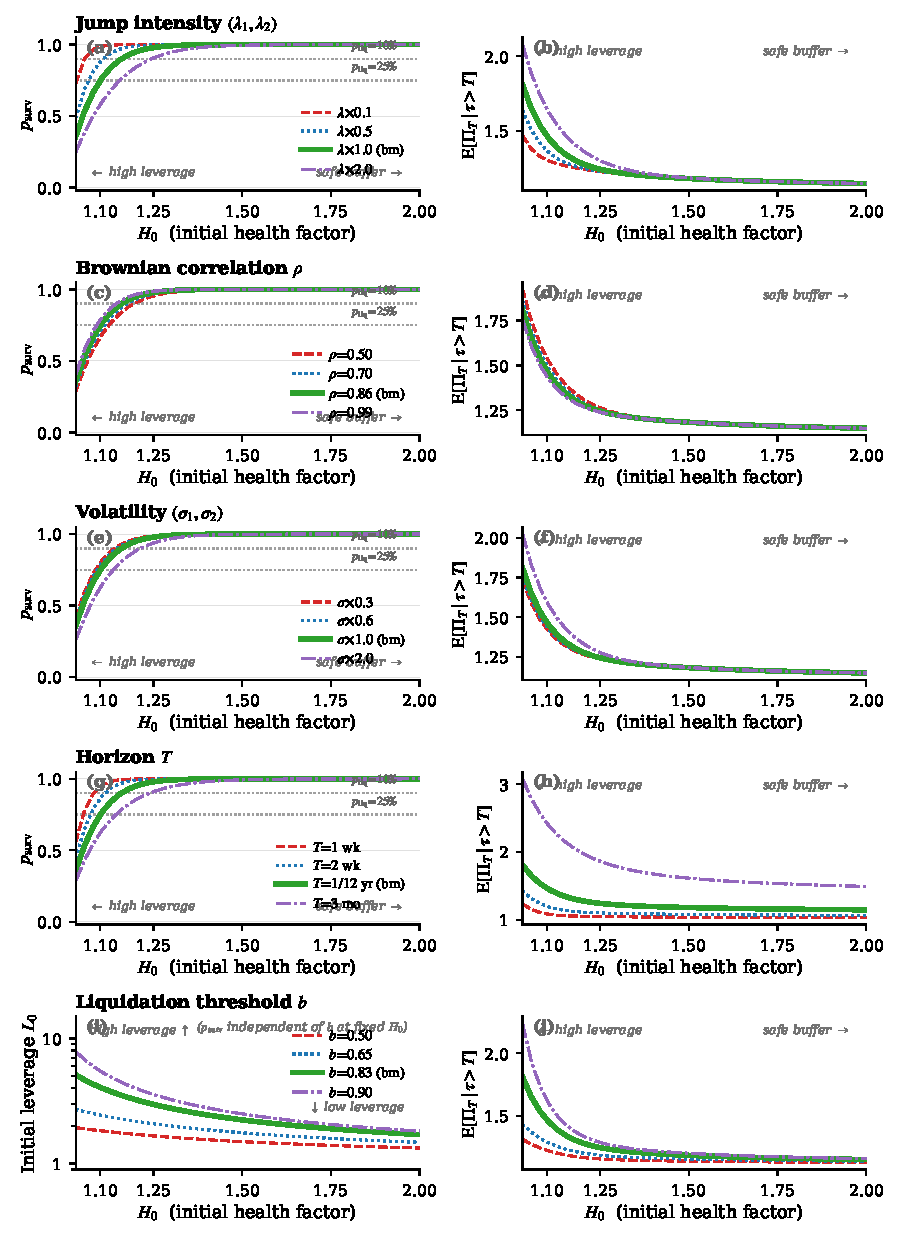
\includegraphics[width=\linewidth,height=0.80\textheight,keepaspectratio]{fig_sensitivity.pdf}
\caption{Left column: survival probability $p_{\mathrm{surv}}$ (rows~a--d) and initial
leverage $L_0$ (row~e, log scale) versus $H_0$. Right column: conditional mean
$\E[\Pi_T\mid\tau>T]$. Each row varies one parameter; all others fixed at
Table~\ref{tab:num-params}. Encoding: colour and line style identify parameter values
(solid/green = benchmark); the heavier line is the baseline.
Laplace--resolvent, $H_0\in[1.068,2.000]$, 40 points per curve.}
\label{fig:sensitivity}
\end{figure}

\clearpage
\subsection{Calibration and sizing uncertainty}\label{sec:calibration-uncertainty}

Pointwise parameter sweeps do not quantify joint sampling variation. We therefore apply a
paired circular moving-block percentile bootstrap to the 540 four-hour return pairs. Each
replicate resamples the same contiguous index blocks for WBTC and WETH, preserving their
contemporaneous pairing and short-range ordering, then repeats ECF calibration, the fixed
AAVE rate adjustment, the fourth-moment admissibility check, and the downstream sizing
rule. The experiment uses 40 replicates, nine-observation blocks (1.5 days), a fixed seed,
and two calibration starts per replicate. All 40 calibrations converged and all 40 sizing
problems were feasible. Two starts make this a tractable uncertainty illustration; the
point calibration itself uses the more extensive 30-start search described in
Appendix~\ref{sec:ecf-init}.

Table~\ref{tab:bootstrap-uncertainty} propagates each recalibration through the rule that
maximizes initial leverage subject to $p_{\mathrm{liq}}\leq0.10$ on the same 200-point
$H_0\in[1.068,2.000]$ grid used below. At the point-selected reference buffer
$H_0=1.274$, survival is $0.902$, while its bootstrap interval is wide. The selected buffer
and leverage also vary materially across recalibrations. By contrast, selected liquidation
probabilities cluster just below 10\% because that is the imposed grid constraint, not
because liquidation risk is precisely estimated.

\begin{table}[ht]
\centering\small
\renewcommand{\arraystretch}{1.2}
\begin{tabular}{lrr}
\toprule
Quantity & Point estimate & 90\% percentile interval \\
\midrule
$p_{\mathrm{surv}}$ at reference $H_0=1.274$ & $0.902$ & $[0.483,\,0.978]$ \\
Selected $H_0$ & $1.274$ & $[1.175,\,1.536]$ \\
Selected initial leverage $L_0$ & $2.577$ & $[2.032,\,2.974]$ \\
Selected $p_{\mathrm{liq}}$ & $0.0980$ & $[0.0943,\,0.0997]$ \\
\bottomrule
\end{tabular}
\caption{Paired circular moving-block bootstrap, conditional on the Kou specification,
penalized ECF criterion, EWM preprocessing, fixed AAVE rates and protocol terms, chosen
block length, and discrete sizing grid. These descriptive intervals measure within-model
sampling variability; they are neither model-selection nor out-of-sample forecast
intervals. Script \texttt{jobs/calibration\_uncertainty.py}.}
\label{tab:bootstrap-uncertainty}
\end{table}

\clearpage
% ============================================================
\section{Application: Initial Health-Buffer Sizing}\label{sec:application}
% ============================================================

The map in \eqref{eq:evaluation-map} can support different initial-buffer rules without
changing the underlying moment calculation. This section gives three examples. They are
deliberately stylized decision rules, not competing claims about the uniquely correct
investor objective.

Write
\[
\mu_c(h_0):=\E[\Pi_T\mid\tau>T],
\qquad
v_c(h_0):=\operatorname{Var}(\Pi_T\mid\tau>T),
\]
and, under the killed-payoff convention,
\[
\mu_u(h_0):=M_1(T,h_0),
\qquad
v_u(h_0):=M_2(T,h_0)-M_1(T,h_0)^2.
\]
The subscripts distinguish moments conditional on survival from unconditional moments of
the random variable that is set to zero after liquidation.

\subsection{Candidate decision rules}

\textit{Liquidation-constrained rule.}
Given a surviving-path score $J_{\mathrm{surv}}$ and a liquidation budget $\bar p$, select
an objective-specific buffer from
\begin{equation}\label{eq:rule-constrained}
\underset{h_0\in\mathcal H(b,\ell_{\max})}{\operatorname{arg\,max}}
\ J_{\mathrm{surv}}(h_0)
\quad\text{subject to}\quad
p_{\mathrm{liq}}(T,h_0)\le \bar p.
\end{equation}
For example, a policy that seeks the greatest initial exposure allowed by a risk limit sets
$J_{\mathrm{surv}}=L_0$.

\textit{Unconditional killed-payoff mean--variance rule.}
For $\alpha\ge0$, select from
\begin{equation}\label{eq:rule-unconditional}
\underset{h_0\in\mathcal H(b,\ell_{\max})}{\operatorname{arg\,max}}
\left\{\mu_u(h_0)-\frac{\alpha}{2}v_u(h_0)\right\}.
\end{equation}
This rule treats the killed payoff as terminal wealth. Its interpretation therefore depends
on the deliberately severe zero-after-liquidation convention and need not coincide with a
criterion based on a protocol recovery model.

\textit{Conditional performance with an explicit liquidation penalty.}
For $\alpha,\delta\ge0$, select from
\begin{equation}\label{eq:Phi}
\underset{h_0\in\mathcal H(b,\ell_{\max})}{\operatorname{arg\,max}}
\left\{\mu_c(h_0)-\frac{\alpha}{2}v_c(h_0)
-\delta p_{\mathrm{liq}}(T,h_0)\right\}.
\end{equation}
Here $\delta$ is an explicit preference parameter, not a quantity identified by the price
model. Conditional moments can also display survivor selection near the barrier; the
penalty controls how the decision rule weighs that feature against liquidation incidence.
The paper does not claim that any one of \eqref{eq:rule-constrained}--\eqref{eq:Phi} is
universally correct. Their purpose is to show how the same semi-analytic outputs enter
different ex-ante preferences.

\subsection{Illustrative evaluation frontier and selected buffers}

Figure~\ref{fig:frontier} reports the baseline evaluation curve. Its primary output is the
mapping from $H_0$ to conditional mean, variance, liquidation probability, and leverage.
The penalized criterion in panel~(d) is one marked use of that curve, rather than the paper's
central result. Table~\ref{tab:objective-comparison} compares several rules on the same
baseline calibration and makes their preference parameters explicit. A selected value at a
candidate-set endpoint is reported as such; it should not be read as an interior or universal
optimum.

\begin{table}[ht]
\centering\small
\renewcommand{\arraystretch}{1.25}
\begin{tabularx}{\linewidth}{@{}Xcccc@{}}
\toprule
Rule & Parameters & Selected $H_0$ & Initial $L_0$ & $p_{\mathrm{liq}}$ \\
\midrule
Maximum leverage under risk limit & $\bar p=0.05$ & $1.331$ & $2.417$ & $0.0478$ \\
Maximum leverage under risk limit & $\bar p=0.10$ & $1.274$ & $2.577$ & $0.0980$ \\
Maximum leverage under risk limit & $\bar p=0.20$ & $1.214$ & $2.799$ & $0.1976$ \\
Unconditional mean--variance & $\alpha=0.5$ & $2.000$ & $1.639$ & $<10^{-4}$ \\
Unconditional mean--variance & $\alpha=1$ & $2.000$ & $1.639$ & $<10^{-4}$ \\
Unconditional mean--variance & $\alpha=5$ & $2.000$ & $1.639$ & $<10^{-4}$ \\
Conditional mean--variance--penalty & $(\alpha,\delta)=(1,0)$ & $1.068$ & $3.704$ & $0.6937$ \\
Conditional mean--variance--penalty & $(\alpha,\delta)=(20,0)$ & $2.000$ & $1.639$ & $<10^{-4}$ \\
Conditional mean--variance--penalty & $(\alpha,\delta)=(1,0.25)$ & $1.068$ & $3.704$ & $0.6937$ \\
Conditional mean--variance--penalty & $(\alpha,\delta)=(1,0.5)$ & $2.000$ & $1.639$ & $<10^{-4}$ \\
\bottomrule
\end{tabularx}
\caption{Objective-specific selections and preference-parameter sensitivity for the
baseline WBTC/WETH illustration over a 200-point grid on
$H_0\in[1.068,2.000]$. Values are computed from the same survival and moment map; only
the decision rule or its stated parameters change. Grid-endpoint selections show why the
table is an illustration rather than evidence of a preferred practical buffer. The
liquidation-constrained rows maximize $L_0$ subject to the stated budget.}
\label{tab:objective-comparison}
\end{table}

\begin{figure}[ht]
\centering
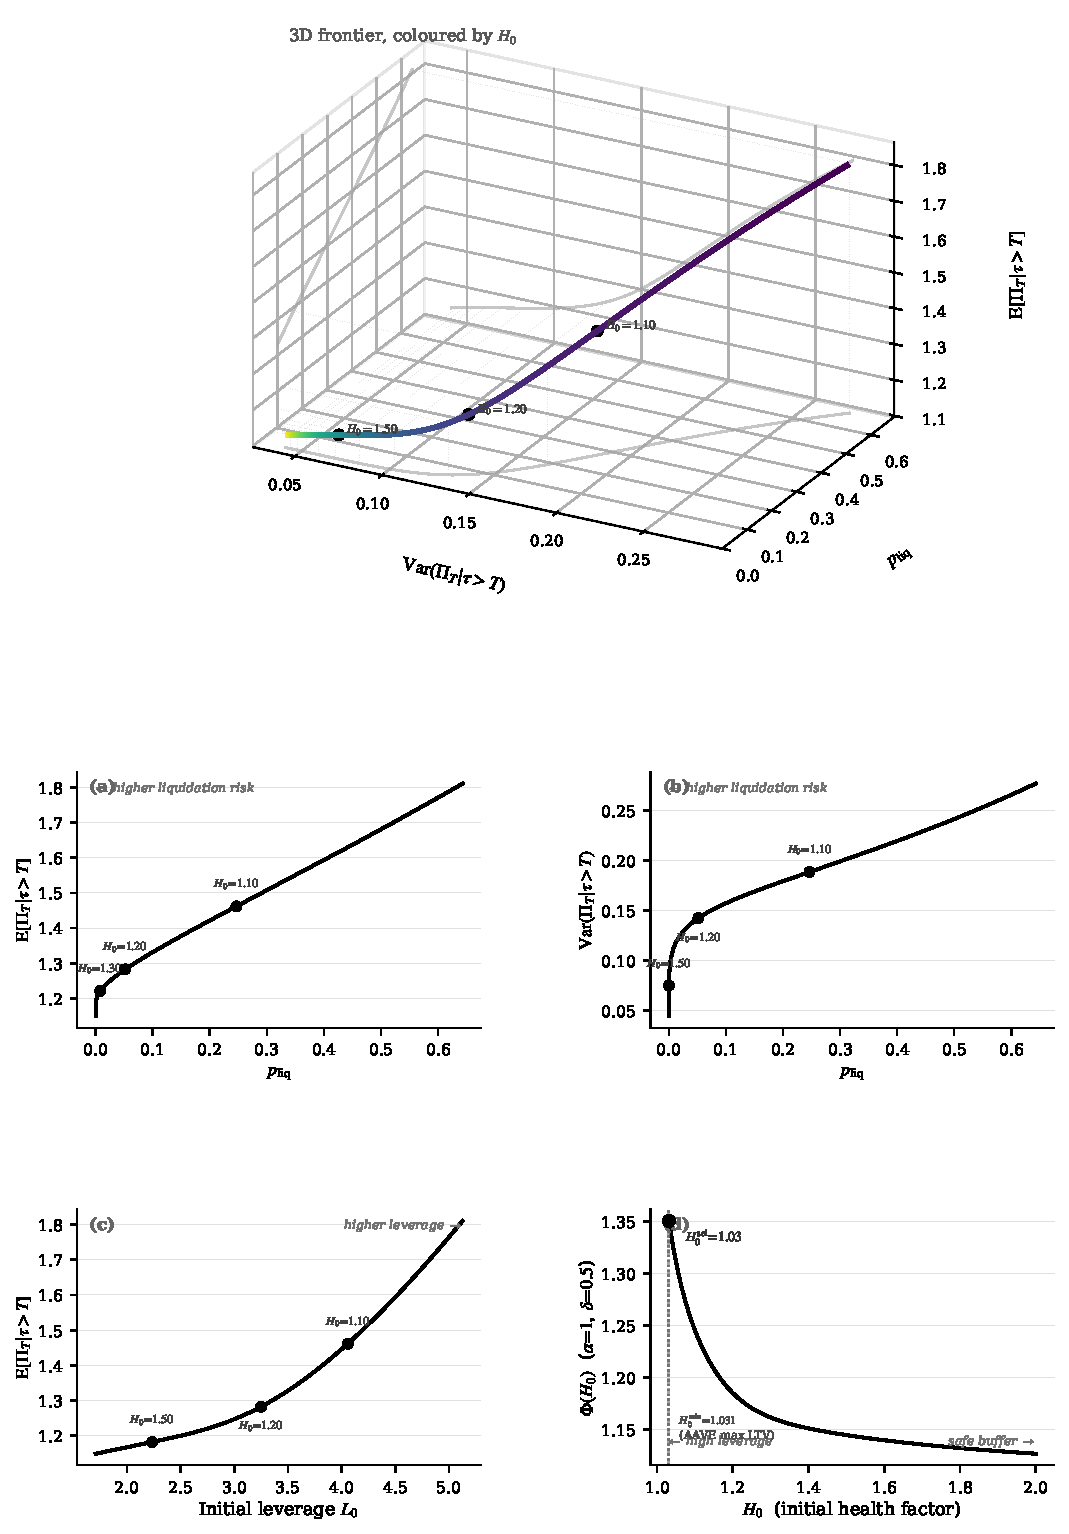
\includegraphics[width=0.92\linewidth]{fig_frontier.pdf}
\caption{Evaluation map for the benchmark parametrisation.
Axes: $x=\mathrm{Var}(\Pi_T\mid\tau>T)$, $y=p_\ell=1-p_{\mathrm{surv}}$,
$z=\mathrm{E}[\Pi_T\mid\tau>T]$ (vertical).
The curve is parametrised by $H_0\in[1.068,2.000]$; the projections show the
mean--liquidation, risk--liquidation, and mean--leverage relationships. Panel~(d) illustrates
the conditional criterion \eqref{eq:Phi} for $(\alpha,\delta)=(1,0.5)$; it is not designated
as the preferred rule. Script \texttt{jobs/frontier\_analysis.py}.}
\label{fig:frontier}
\end{figure}

% ============================================================
\section{Conclusion and Discussion}\label{sec:discussion}
% ============================================================

We derive an exact Laplace-domain representation and a semi-analytic numerical procedure
for survival probabilities and killed payoff moments of a leveraged crypto long--short
position whose liquidation boundary is determined by a collateral-to-liability ratio. The
initial
log health factor reduces the holdings to one parameter, and an exponential measure change
reduces each fixed admissible integer-order moment to a killed expectation of the log-price
ratio. Under Kou jump--diffusion dynamics and distinct downward phase rates, three barrier
conditions give a $3\times3$ resolvent system.

These objective-independent quantities turn initial-buffer sizing into a one-dimensional
optimization: rapid evaluation of survival and killed-moment outputs supports buffer
selection under alternative liquidation constraints and moment-based preferences. The
numerical results compare the resolvent output with discretely monitored Monte Carlo,
verify the analytical no-shorting limit, and illustrate sensitivity across model and
contract inputs. The paired block bootstrap further shows that within-model calibration
uncertainty can materially shift the selected buffer, so the optimal buffer moves with the
objective, its risk parameters, the loss convention, and the calibration itself; no single
selection should be read as a universal practical optimum.

The model omits liquidation recovery, dynamic collateral intervention, oracle and keeper
delays, stochastic borrowing rates, execution costs, and market impact. Incorporating these
features would change investor terminal wealth and may change the selected buffer. The
principal output is therefore not a single leverage number, but the map from the initial
health buffer to survival probability and payoff-distribution characteristics -- the input
that any sizing rule, whether the illustrative ones used here or a more complete dynamic
control model, ultimately needs to solve for the optimal buffer.

\clearpage
\appendices

% ============================================================
\section{Empirical Calibration}\label{sec:calibration}
% ============================================================

\subsection{Estimator}\label{sec:ecf-estimator}

The bivariate Kou model admits the closed-form Lévy--Khintchine exponent
$\Psi(u,v)$ derived in Section~\ref{sec:model}, so no numerical density
inversion is required to compute the model-implied characteristic function
\begin{equation}\label{eq:model-cf}
\phi_\theta(u,v;\Delta)
=
\exp\!\bigl(\Delta\,\Psi_\theta(u,v)\bigr),
\end{equation}
where $\Delta$ is the observation interval.
Given $N$ observed bivariate log-return pairs $(r_{1,n},r_{2,n})_{n=1}^N$,
the empirical characteristic function is
\begin{equation}\label{eq:ecf}
\widehat{\phi}_N(u,v)
=
\frac{1}{N}\sum_{n=1}^N
\exp\!\bigl(i(u\,r_{1,n}+v\,r_{2,n})\bigr).
\end{equation}
The ECF component of the estimator is the normalized weighted squared distance
between \eqref{eq:ecf} and \eqref{eq:model-cf} over a discrete frequency grid
$\mathcal{G}$:
\begin{equation}\label{eq:ecf-objective}
Q_N^{\mathrm{ECF}}(\theta)
=
\frac{\displaystyle\sum_{(u,v)\in\mathcal{G}}w(u,v)
\,\bigl|\widehat{\phi}_N(u,v)-\phi_\theta(u,v;\Delta)\bigr|^2}
{\displaystyle\sum_{(u,v)\in\mathcal{G}}w(u,v)}.
\end{equation}
Because finite high-frequency samples leave a pronounced intensity--jump-size ridge, the
reported calibration uses two transparent soft anchoring terms:
\begin{equation}\label{eq:ecf-penalized-objective}
\begin{aligned}
\widehat{\theta}
&=\arg\min_{\theta\in\Theta}\mathcal{Q}_N(\theta),\\
\mathcal{Q}_N(\theta)
&=Q_N^{\mathrm{ECF}}(\theta)
+\omega_\lambda\sum_{i=1}^{2}(\log\lambda_i-\log\widetilde\lambda_i)^2\\
&\quad+\omega_\eta\sum_{i=1}^{2}\sum_{s\in\{+,-\}}
(\log\eta_{i,s}-\log\widetilde\eta_{i,s})^2.
\end{aligned}
\end{equation}
Here $\widetilde\lambda_i$ is the variance/fourth-cumulant initializer and
$\widetilde\eta_{i,s}$ is the peak-over-threshold (POT) mean-excess initializer described
below. The application uses $(\omega_\lambda,\omega_\eta)=(0.05,0.02)$. These are soft
penalties, not equality restrictions; setting both weights to zero recovers pure ECF
matching.
This is the empirical-characteristic-function approach of
\citet{Singleton2001}, which is particularly natural for affine and
Lévy-based asset-pricing models whose characteristic functions are known in
closed form.
\citet{FeuervergerMcDunnough1981} establish that ECF estimators over a
rich grid can attain maximum-likelihood efficiency.
The procedure avoids evaluating the bivariate transition density, which would
require a two-dimensional numerical Fourier inversion inside every optimizer
call.
For background on DEJD likelihood estimation in the univariate case
see \citet{RamezaniZeng2007}.

\subsection{Frequency grid}\label{sec:ecf-grid}

The parameter vector $\theta$ has $13$ free components; see Table~\ref{tab:params}.
Raw return magnitudes depend on the sampling interval, so fixed raw Fourier frequencies
are poorly portable. Let $s_1$, $s_2$, and $s_Z$ be IQR-based robust scales,
$s=\max\{(q_{0.75}-q_{0.25})/1.349,10^{-8}\}$, for $r_1$, $r_2$, and $r_1-r_2$. Dimensionless base
frequencies are mapped to raw frequencies by division by the corresponding scale. The
grid contains the following groups, with every point accompanied by its conjugate
$(-u,-v)$:
\begin{itemize}
  \item marginal points $(a/s_1,0)$ and $(0,a/s_2)$ for
    $a\in\mathcal{A}_{\mathrm{marg}}$;
  \item same-sign and mixed-sign joint points
    $(a/s_1,b/s_2)$ and $(a/s_1,-b/s_2)$ for
    $a,b\in\mathcal{A}_{\mathrm{joint}}$, which are informative about $\rho$;
  \item spread points $(a/s_Z,-a/s_Z)$ for $a\in\mathcal{A}_Z$, which directly
    match the log-ratio process governing liquidation; and
  \item high-base marginal and spread points for $a\in\mathcal{A}_{\mathrm{tail}}$,
    included to retain information about jump-tail shape.
\end{itemize}
The dimensionless base nodes are
\begin{align*}
\mathcal{A}_{\mathrm{marg}}&=\{0.1,0.2,0.5,0.75,1,1.5,2,3,5,7.5,10\},\\
\mathcal{A}_{\mathrm{joint}}&=\{0.25,0.5,1,2,3,5\},\\
\mathcal{A}_{Z}&=\{0.1,0.2,0.5,0.75,1,1.5,2,3,5\},\\
\mathcal{A}_{\mathrm{tail}}&=\{8,12,16,20,25\}.
\end{align*}
Points whose absolute raw coordinate exceeds $5{,}000$ are discarded to avoid numerical
aliasing. Including conjugate pairs, the unfiltered construction has 236 frequency
evaluations; this cap leaves 234 for the application sample. Weights depend on dimensionless
rather than raw frequency:
\[
w(a,b)=\exp\{-0.02(a^2+b^2)\}.
\]
The ordinary spread group receives an additional factor of two. Thus the criterion
emphasizes the barrier-driving ratio without making the choice of observation interval
determine the effective frequency weights.

\subsection{Reparameterisation and initialisation}\label{sec:ecf-init}

\paragraph{Unconstrained reparameterisation.}
Constraints in Table~\ref{tab:params} are enforced automatically via the
change of variables
\begin{equation}\label{eq:reparam}
\sigma_i=e^{a_i},\quad
\lambda_i=e^{b_i},\quad
p_i=\mathrm{sigmoid}(c_i),\quad
\eta_{i,+}=\eta_{i,+}^{\max}\mathrm{sigmoid}(d_i),\quad
\eta_{i,-}=e^{e_i},\quad
\rho=\tanh(f),
\end{equation}
where sigmoid$(x)=(1+e^{-x})^{-1}$.
The unconstrained vector $\tau=({\mu_1,a_1,b_1,c_1,d_1,e_1,\mu_2,\ldots,f})$
is optimized with box bounds in this transformed space. For both assets the code uses
a scaled sigmoid with
\[
\eta_{i,+}^{\max}\le (1-\varepsilon)/K,
\qquad i=1,2,
\]
so that both moment-admissibility conditions in \eqref{eq:moment-admissibility}
are enforced directly through order $K$.

\paragraph{Threshold initialiser.}
The characteristic-function objective is non-linear and non-convex,
so the optimisation is initialised by a threshold-based decomposition
following the logic of \citet{Mancini2009} for discretely observed
jump-diffusions.
Let $m_i=\mathrm{median}(r_{i,n})$ and let $s_i$ be the IQR robust scale.
For a frequency-aware threshold constant $c\in[3,5]$, define candidate
jump observations
\[
\mathcal{J}_i=\{n:|r_{i,n}-m_i|>c\,s_i\},
\qquad
\mathcal{C}_i=\{1,\ldots,N\}\setminus\mathcal{J}_i.
\]
Initial volatility and correlation values use the continuous subset
$\mathcal{C}_i$, while the jump-size means are anchored by peak-over-threshold
excess means and the intensities are corrected by a variance/fourth-cumulant
estimate.  Schematically:
\begin{align*}
p_i^{(0)}&=\frac{|\mathcal{J}_{i,+}|}{|\mathcal{J}_i|}
  \quad\text{clamped to the admissible probability range},\\
\eta_{i,+}^{(0)},\,\eta_{i,-}^{(0)}&=\text{POT mean-excess estimates},\\
\lambda_i^{(0)}&=\text{two-moment estimate from variance and fourth cumulant},\\
\sigma_i^{(0)}&=\mathrm{sd}(r_{i,n}:\,n\in\mathcal{C}_i)/\sqrt{\Delta},
&
\rho^{(0)}&=\mathrm{corr}(r_1,r_2)_{n\in\mathcal{C}_1\cap\mathcal{C}_2}.
\end{align*}
The initializer first estimates the annualized log-process drift with a damped
mean-jump correction,
\[
\mu_i^{X,(0)}=\bar{r}_i/\Delta
-0.25\,\lambda_i^{(0)}
\left[p_i^{(0)}\eta_{i,+}^{(0)}-(1-p_i^{(0)})\eta_{i,-}^{(0)}\right],
\]
then stores the result in the paper's price-growth convention,
\[
\mu_i^{(0)}=\operatorname{clip}_{[\mu_{\min},\mu_{\max}]}
\!\left(\mu_i^{X,(0)}+\tfrac12(\sigma_i^{(0)})^2
+\lambda_i^{(0)}\chi_i^{(0)}\right).
\]
The threshold filter is not the final estimator.
It is a warm start that places the optimizer in a sensible region of
parameter space; see the remark in \citet{Mancini2009}.

\paragraph{Multi-start cloud.}
Because $\mathcal{Q}_N(\tau)$ may have local minima, the optimizer is run from a
structured cloud. It contains the unperturbed initializer and six deterministic
intensity--size ridge starts with
\[
\lambda_i\mapsto c\lambda_i,\qquad
\eta_{i,\pm}\mapsto\eta_{i,\pm}/\sqrt{c},qquad
c\in\{0.1,0.25,0.5,2,4,8\}.
\]
Remaining starts cycle through four high-jump/high-diffusion scenarios and add bounded
random perturbations to scale, probability, correlation, and drift parameters. The
application calibration uses 30 starts (the library default is 20) and returns the bounded
L-BFGS-B minimizer with the lowest penalized objective.

\subsection{Identifiability and model-comparison protocol}\label{sec:ecf-ident}

The penalized criterion $\mathcal{Q}_N(\theta)$ is non-convex.
Jump-diffusion models possess approximate ridges along directions that
preserve the compound-Poisson variance contribution
$\lambda_i\E[J_i^2]=2\lambda_i(p_i\eta_{i,+}^2+(1-p_i)\eta_{i,-}^2)$
\citep{RamezaniZeng2007}.
The diffusion volatilities $\sigma_i$ and the Brownian correlation $\rho$
are generally better identified from short samples than jump-size and intensity
parameters, which carry larger finite-sample uncertainty unless the observation
window contains many jump events. Because $\lambda_i$ is annualized, a one-year
window contains $\lambda_i$ jumps in expectation, irrespective of whether prices
are sampled hourly or daily. Finer sampling can make individual jumps easier to
separate from aggregated returns, but it does not multiply the underlying annual
Poisson count.

For descriptive fit comparisons on a common grid, compare the unpenalized component
$Q_N^{\mathrm{ECF}}(\widehat\theta)$ across nested models (GBM, Merton, bivariate Kou),
rather than the penalized values $\mathcal{Q}_N(\widehat\theta)$ whose anchors differ.
Such comparisons should be accompanied by liquidation-relevant diagnostics:
empirical versus model $Z$-tail quantiles, empirical versus model
barrier-crossing frequencies, and simulated versus observed drawdowns of $Z$.
These are more directly informative for the sizing application than
standard likelihood-based criteria.
The present numerical illustration does not carry out a formal GBM--Merton--Kou selection
exercise. It does propagate within-model sampling variability through the paired circular
moving-block bootstrap reported in Section~\ref{sec:calibration-uncertainty}. Those intervals
remain conditional on the selected Kou model and stated empirical choices; they are not
evidence of model dominance or parameter-robust recommendations.

The repository's calibration package contains the implementation. The
synthetic calibration job shows parameter recovery and produces
Figure~\ref{fig:ecf-fit}.

\begin{figure}[ht]
\centering
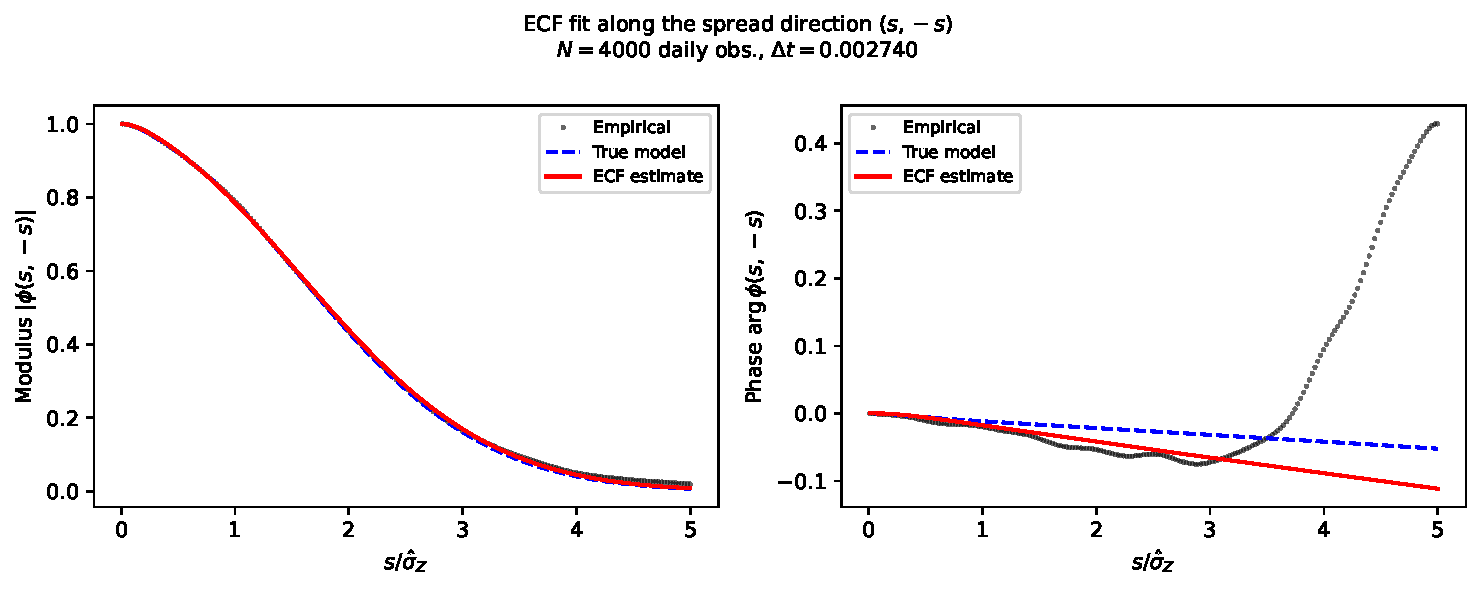
\includegraphics[width=0.85\linewidth]{fig_ecf_fit.pdf}
\caption{ECF fit along the spread direction $(s,-s)$ for $N=4{,}000$
synthetic daily log-return observations.
Left: modulus $|\phi(s,-s)|$; right: phase $\arg\phi(s,-s)$.
Dots: empirical CF $\widehat\phi_N$; dashed: true model CF;
solid red: ECF estimate.
The close agreement in modulus and phase documents the fit along the
liquidation-relevant spread direction; this plot alone does not assess every component of
the full-grid criterion.
Script \texttt{jobs/calibrate\_kou.py}.}
\label{fig:ecf-fit}
\end{figure}

\clearpage
% ============================================================
\section{Killing at the Barrier and Downward-Phase Corrections}
\label{app:downward-phases}
% ============================================================

Section~\ref{sec:resolvent} uses only the generator $\mathcal L^{(k)}$ from
Lemma~\ref{lem:psiZk}, with a killed expectation extended by zero below the barrier. This
appendix records how that convention changes the downward jump integrals and derives the
three rows of the barrier system \eqref{eq:barrier-system}.

\subsection{Phase Operators and Zero Extension}

\begin{definition}[Phase operators]\label{def:phase-ops}
For $j=1,2$, the phase operators associated with the tilted jump kernels of $Z$ under
$\P^{(k)}$ are
\[
K_{j,+}^{(k)}[f](x)
:=
\int_0^\infty f(x+y)r_{j,+}^{(k)}e^{-r_{j,+}^{(k)}y}\,\diff y,
\qquad
K_{j,-}^{(k)}[f](x)
:=
\int_0^\infty f(x-y)r_{j,-}^{(k)}e^{-r_{j,-}^{(k)}y}\,\diff y.
\]
For any complex $\gamma$ with
$\Rea(\gamma)<r_{j,+}^{(k)}$ and $\Rea(\gamma)>-r_{j,-}^{(k)}$, direct integration gives
\begin{equation}\label{eq:phase-on-exp}
K_{j,+}^{(k)}[e^{\gamma\cdot}](x)
=
\frac{r_{j,+}^{(k)}}{r_{j,+}^{(k)}-\gamma}e^{\gamma x},
\qquad
K_{j,-}^{(k)}[e^{\gamma\cdot}](x)
=
\frac{r_{j,-}^{(k)}}{r_{j,-}^{(k)}+\gamma}e^{\gamma x}.
\end{equation}
\end{definition}
This phase construction originates in \citet{KouWang2003} for first-passage problems under
the double-exponential model and is used by \citet{Sepp2004} to reduce barrier pricing to a
finite linear system.

The tilted phase intensities are
\begin{equation}\label{eq:tilted-intensities}
\lambda_{1,+}^{(k)}=\lambda_1p_1,
\quad
\lambda_{1,-}^{(k)}=\lambda_1(1-p_1),
\quad
\lambda_{2,+}^{(k)}=\frac{\lambda_2(1-p_2)}{1+k\eta_{2,-}},
\quad
\lambda_{2,-}^{(k)}=\frac{\lambda_2p_2}{1-k\eta_{2,+}}.
\end{equation}
Using Definition~\ref{def:phase-ops}, the full-line action of the generator is
\begin{equation}\label{eq:generic-generator}
\mathcal L^{(k)}f(x)
=\mu_Z^{(k)}f'(x)+\frac{\sigma_Z^2}{2}f''(x)
+\sum_{a=1}^2\lambda_{a,+}^{(k)}\bigl(K_{a,+}^{(k)}[f](x)-f(x)\bigr)
+\sum_{d=1}^2\lambda_{d,-}^{(k)}\bigl(K_{d,-}^{(k)}[f](x)-f(x)\bigr).
\end{equation}
Applying \eqref{eq:phase-on-exp} recovers the exponential symbol
\eqref{eq:generator-eigen}.

Now let $f$ be defined on the alive half-line $x>0$ and let
$\bar f=f\one_{(0,\infty)}$ be its zero extension. Upward jumps remain in the alive region,
whereas a downward jump of size $y\ge x$ lands in the absorbing region. Consequently,
\begin{equation}\label{eq:killed-downward-operator}
K_{d,-}^{(k)}[\bar f](x)
=K_{d,-}^{(k),D}[f](x)
:=\int_0^x f(x-y)r_{d,-}^{(k)}e^{-r_{d,-}^{(k)}y}\,\diff y,
\qquad x>0.
\end{equation}
Substitution into \eqref{eq:generic-generator} gives
\begin{equation}\label{eq:zero-extended-generator}
\begin{aligned}
\mathcal L^{(k)}[\bar f](x)
={}&\mu_Z^{(k)}f'(x)+\frac{\sigma_Z^2}{2}f''(x)
+\sum_{a=1}^2\lambda_{a,+}^{(k)}
  \bigl(K_{a,+}^{(k)}[f](x)-f(x)\bigr)\\
&+\sum_{d=1}^2\lambda_{d,-}^{(k)}
  \bigl(K_{d,-}^{(k),D}[f](x)-f(x)\bigr),
\qquad x>0.
\end{aligned}
\end{equation}
Thus killing changes the arguments on which $\mathcal L^{(k)}$ acts, not the identity of the
generator. Equation~\eqref{eq:zero-extended-generator} is the standard zero-extension
construction for a L\'evy process killed at an absorbing boundary.

\subsection{Downward-Phase Residual and Barrier Conditions}

\begin{lemma}[Truncated downward phase]\label{lem:truncated-phase}
For $r>0$, $\beta\in\mathbb C\setminus\{-r\}$, and $x>0$,
\begin{equation}\label{eq:truncated-phase}
\int_0^x e^{\beta(x-y)}r e^{-ry}\,\diff y
=\frac{r}{r+\beta}e^{\beta x}
-\frac{r}{r+\beta}e^{-rx}.
\end{equation}
No restriction $\Rea(\beta)>-r$ is needed, since the integral is over a finite interval.
\end{lemma}
\proofref{proof:lem:truncated-phase}

For a finite exponential sum $v(x)=\sum_{\beta\in\mathcal E}a_\beta e^{\beta x}$, define
the truncation-correction coefficient
\begin{equation}\label{eq:correction-functional}
\mathfrak C_r[v]
:=\sum_{\beta\in\mathcal E}a_\beta\frac{r}{r+\beta}.
\end{equation}
Then \eqref{eq:truncated-phase} gives
\begin{equation}\label{eq:truncated-decomposition}
K_{r,-}^{D}[v](x)
:=\int_0^x v(x-y)re^{-ry}\,\diff y
=\sum_{\beta\in\mathcal E}a_\beta\frac{r}{r+\beta}e^{\beta x}
-\mathfrak C_r[v]e^{-rx}.
\end{equation}
Combining \eqref{eq:zero-extended-generator} and
\eqref{eq:truncated-decomposition}, for exponents at which the upward integrals are finite
and which avoid the downward phase poles,
\begin{equation}\label{eq:zero-extension-residual}
\mathcal L^{(k)}[\bar v](x)
=\sum_{\beta\in\mathcal E}a_\beta\psi_Z^{(k)}(\beta)e^{\beta x}
-\sum_{d=1}^2\lambda_{d,-}^{(k)}
  \mathfrak C_{r_{d,-}^{(k)}}[v]e^{-r_{d,-}^{(k)}x},
\qquad x>0,
\end{equation}
where $\psi_Z^{(k)}$ is understood through the meromorphic continuation of its exponential
symbol outside the common full-line moment strip.

Apply \eqref{eq:zero-extension-residual} term by term to the interior ansatz
\eqref{eq:interior-ansatz}. Its forcing coefficients and characteristic-root equations give
\begin{equation}\label{eq:killed-residual}
(q-\mathcal L^{(k)})\widehat U_k(q,x)
=G_k(x)
+\sum_{d=1}^2\lambda_{d,-}^{(k)}
  \mathfrak C_{r_{d,-}^{(k)}}[\widehat U_k(q,\cdot)]
  e^{-r_{d,-}^{(k)}x}.
\end{equation}
When the two downward rates are distinct, the residual exponentials are linearly
independent, so the interior equation holds if and only if both correction coefficients
vanish. Since $\sigma_Z>0$, the lower boundary is regular for the Brownian component and
absorption also imposes the Dirichlet condition. The three conditions are therefore
\begin{equation}\label{eq:three-barrier-conditions}
\widehat U_k(q,0)=0,
\qquad
\mathfrak C_{r_{1,-}^{(k)}}[\widehat U_k(q,\cdot)]=0,
\qquad
\mathfrak C_{r_{2,-}^{(k)}}[\widehat U_k(q,\cdot)]=0.
\end{equation}
Substituting \eqref{eq:interior-ansatz} into \eqref{eq:three-barrier-conditions} gives
\[
\sum_{m=1}^3B_m^{(k)}
=-\sum_{j=0}^{k}\frac{d_{k,j}}{q-\psi_Z^{(k)}(j)},
\]
and, for $d=1,2$,
\[
\sum_{m=1}^3
\frac{r_{d,-}^{(k)}}{r_{d,-}^{(k)}+\gamma_{m+3}^{(k)}(q)}B_m^{(k)}
=-\sum_{j=0}^{k}\frac{d_{k,j}}{q-\psi_Z^{(k)}(j)}
  \frac{r_{d,-}^{(k)}}{r_{d,-}^{(k)}+j}.
\]
These are precisely the three rows of \eqref{eq:barrier-system}.

\begin{lemma}[Invertibility of $\mathbf{M}_{\mathrm{bar}}^{(k)}(q)$]\label{lem:Mbar-inv}
Under Assumption~\ref{ass:six-root} and condition~\eqref{eq:nondeg-bar}, the barrier matrix
$\mathbf{M}_{\mathrm{bar}}^{(k)}(q)$ in \eqref{eq:barrier-matrix} is invertible.
\end{lemma}
\proofref{proof:lem:Mbar-inv}

\begin{remark}[Coincident downward rates]\label{rem:coincident-rates}
If $r_{1,-}^{(k)}=r_{2,-}^{(k)}=:r$, the two downward kernels combine into a single phase.
The meromorphic symbol must first be reduced by cancelling the repeated phase factor;
otherwise clearing denominators introduces a spurious root at the pole $-r$. The reduced
characteristic equation has two genuine decaying roots, say
$\gamma_4^{(k)}(q),\gamma_5^{(k)}(q)$, and the
conditions $\widehat U_k(q,0)=0$ and
$\mathfrak C_r[\widehat U_k(q,\cdot)]=0$ give the $2\times2$ system
\[
\begin{pmatrix}
1&1\\[4pt]
\dfrac{r}{r+\gamma_4^{(k)}(q)}&\dfrac{r}{r+\gamma_5^{(k)}(q)}
\end{pmatrix}
\begin{pmatrix}B_1^{(k)}\\B_2^{(k)}\end{pmatrix}
=-
\begin{pmatrix}
\displaystyle\sum_{j=0}^{k}\frac{d_{k,j}}{q-\psi_Z^{(k)}(j)}\\[10pt]
\displaystyle\sum_{j=0}^{k}\frac{d_{k,j}}{q-\psi_Z^{(k)}(j)}\frac{r}{r+j}
\end{pmatrix}.
\]
Thus the $3\times3$ description applies to the generic distinct-rate regime; the
coincident-rate case is a genuine lower-dimensional phase model, not a singular generic
system.
\end{remark}

\clearpage
% ============================================================
\section{Proofs}\label{app:proofs}
% ============================================================

\begin{proof}[Proof of Lemma~\ref{lem:psiZk}]\label{proof:lem:psiZk}
\textit{Step 1: Laplace transform under $\P^{(k)}$.}
Because $Z_t = X_{1,t}-X_{2,t}$ and the density on $\mathcal{F}_t$ equals
$e^{kX_{2,t}-t\Psi(0,-ik)}$,
\begin{equation}\label{eq:mgf-tilted}
\E_{\P^{(k)}}\!\left[e^{sZ_t}\right]
=
e^{-t\Psi(0,-ik)}\,
\E_\P\!\left[e^{s X_{1,t}+(k-s)X_{2,t}}\right]
=
e^{t\left[\Psi(-is,-i(k-s))-\Psi(0,-ik)\right]},
\end{equation}
where we used $\E_\P[e^{\alpha X_{1,t}+\beta X_{2,t}}]=e^{t\Psi(-i\alpha,-i\beta)}$.
This identity is first valid for $s$ in the common moment-generating strip.  In particular,
$k\eta_{2,+}<1$ is needed at $s=0$ to define the tilt, and evaluating the payoff forcing at
$s=j$, $j=0,\ldots,k$, additionally requires $k\eta_{1,+}<1$.
Since the Radon--Nikod\'ym density is exponential-linear in $(X_{1,t},X_{2,t})$, Girsanov's theorem
for L\'evy processes guarantees that $Z$ remains a L\'evy process under $\P^{(k)}$ with exponent
\begin{equation}\label{eq:psiZk-raw}
\psi_Z^{(k)}(s) = \Psi\!\left(-is,\,-i(k-s)\right)-\Psi(0,-ik).
\end{equation}

\textit{Step 2: Expand and simplify.}
Substituting \eqref{eq:Psi} with $(u,v)=(-is,-i(k-s))$, and noting
$u^2=-s^2$, $v^2=-(k-s)^2$, $uv=-s(k-s)$, and $\varphi_{J_i}(-i\cdot)=M_i(\cdot)$:
\begin{equation}\label{eq:Psi-expanded}
\begin{aligned}
\Psi(-is,-i(k-s))
={}&\mu_1^X s + \mu_2^X(k-s)
+\tfrac12\sigma_1^2 s^2+\tfrac12\sigma_2^2(k-s)^2+\rho\sigma_1\sigma_2 s(k-s)\\
&+\lambda_1(M_1(s)-1)+\lambda_2(M_2(k-s)-1).
\end{aligned}
\end{equation}
Setting $s=0$ in \eqref{eq:Psi-expanded} gives
$\Psi(0,-ik)=\mu_2^X k + \tfrac12\sigma_2^2 k^2 + \lambda_2(M_2(k)-1)$.
Subtracting and collecting terms by type:

\smallskip
\noindent\textit{Drift.}
$\mu_1^X s + \mu_2^X(k-s) - \mu_2^X k
= (\mu_1^X-\mu_2^X)s$.

\smallskip
\noindent\textit{Diffusion.}
Expanding $(k-s)^2 = k^2-2ks+s^2$ and $(k-s) = k-s$:
\begin{align*}
&\tfrac12\sigma_1^2 s^2+\tfrac12\sigma_2^2(k-s)^2+\rho\sigma_1\sigma_2 s(k-s)
-\tfrac12\sigma_2^2 k^2\\
&\quad =\tfrac12(\sigma_1^2+\sigma_2^2-2\rho\sigma_1\sigma_2)s^2
-k(\sigma_2^2-\rho\sigma_1\sigma_2)s
= \tfrac12\sigma_Z^2 s^2 - k(\sigma_2^2-\rho\sigma_1\sigma_2)s.
\end{align*}

\smallskip
\noindent\textit{Jumps.}
$\lambda_1(M_1(s)-1)+\lambda_2(M_2(k-s)-1)-\lambda_2(M_2(k)-1)
=\lambda_1(M_1(s)-1)+\lambda_2(M_2(k-s)-M_2(k))$.

\smallskip
Combining, the drift coefficient is
$\mu_Z^{(k)}:=(\mu_1^X-\mu_2^X)-k(\sigma_2^2-\rho\sigma_1\sigma_2)$,
which establishes \eqref{eq:psiZk}.
The eigenrelation \eqref{eq:generator-eigen} follows because for any L\'evy process with
exponent $\psi$, the generator satisfies $\mathcal{L} e^{sz}=\psi(s)\,e^{sz}$, as can be
seen by differentiating $\E[e^{sZ_t}]=e^{t\psi(s)}$ with respect to $t$ at $t=0$.
\end{proof}

\begin{proof}[Proof of Lemma~\ref{lem:truncated-phase}]\label{proof:lem:truncated-phase}
Direct integration over the finite interval gives
\[
\int_0^x e^{\beta(x-y)}r e^{-ry}\,\diff y
=e^{\beta x}r\int_0^x e^{-(r+\beta)y}\,\diff y
=e^{\beta x}\frac{r}{r+\beta}\bigl(1-e^{-(r+\beta)x}\bigr),
\]
which is \eqref{eq:truncated-phase}. Since the interval is finite, this calculation is valid
for every $\beta\neq-r$ without a full-line integrability condition.
\end{proof}

\begin{proof}[Proof of Proposition~\ref{prop:Ubar}]\label{proof:prop:Ubar}
For the ansatz \eqref{eq:interior-ansatz}, the zero-extension identity
\eqref{eq:killed-residual} shows that the interior resolvent equation holds precisely when
its two downward-phase correction coefficients vanish. Absorption adds
$\widehat U_k(q,0)=0$, giving the three conditions \eqref{eq:three-barrier-conditions}. As
shown in Appendix~\ref{app:downward-phases}, substitution of the ansatz produces exactly the system
\eqref{eq:barrier-system} with matrix \eqref{eq:barrier-matrix} and forcing vector
\eqref{eq:barrier-forcing}. Lemma~\ref{lem:Mbar-inv} gives the unique coefficient vector.

The resulting zero extension solves \eqref{eq:resolvent}; uniqueness of the killed resolvent
in the relevant exponential-growth class identifies it with $\widehat U_k$. Finally,
\eqref{eq:target-transform} and evaluation at $x=h_0$ give \eqref{eq:Uhat-zero}.
\end{proof}

\begin{proof}[Proof of Lemma~\ref{lem:Mbar-inv}]\label{proof:lem:Mbar-inv}
For brevity, write $\gamma_m:=\gamma_m^{(k)}(q)$.  Subtracting row~1 from rows~2 and~3
replaces entry $(i,m)$ for $i=2,3$ by
\[
-\frac{\gamma_{m+3}}{r_{i-1,-}^{(k)}+\gamma_{m+3}}.
\]
Pulling out $-1$ from each of these two rows (net sign $(-1)^2=1$) and then factoring
$\gamma_{m+3}$ from each column gives
\[
\det\!\bigl(\mathbf{M}_{\mathrm{bar}}^{(k)}\bigr)
=
\gamma_4\gamma_5\gamma_6\;
\det\!\left(\frac{1}{x_i+\gamma_{j+3}}\right)_{\!1\le i,j\le 3},
\]
where $x_1:=0$, $x_2:=r_{1,-}^{(k)}$, $x_3:=r_{2,-}^{(k)}$.
The right-hand factor is a Cauchy determinant; the Cauchy formula yields
\[
\det\!\left(\frac{1}{x_i+\gamma_{j+3}}\right)
=
\frac{\prod_{1\le i<i'\le 3}(x_{i'}-x_i)\cdot
      \prod_{4\le m<m'\le 6}(\gamma_{m'}-\gamma_m)}
     {\prod_{i=1}^3\prod_{m=4}^6(x_i+\gamma_m)}.
\]
Since $x_1=0$, the factor $\prod_{m=4}^6(x_1+\gamma_m)=\gamma_4\gamma_5\gamma_6$
cancels with the prefactor, yielding a ratio whose every factor is nonzero:
$r_{1,-}^{(k)}>0$ since $\eta_{1,-}>0$;
$r_{2,-}^{(k)}>0$ since $k\eta_{2,+}<1$;
$(r_{2,-}^{(k)}-r_{1,-}^{(k)})\neq 0$ by~\eqref{eq:nondeg-bar};
the $\gamma_m$ are pairwise distinct by Assumption~\ref{ass:six-root}(ii);
and $r_{j,-}^{(k)}+\gamma_m\neq 0$ because $-r_{j,-}^{(k)}$ is a pole of $\psi_Z^{(k)}$,
so $\psi_Z^{(k)}(-r_{j,-}^{(k)})=\infty\neq q$, hence $\gamma_m\neq -r_{j,-}^{(k)}$.
\end{proof}

The survival probability requires no separate proof: it is the $k=0$ instance of
Proposition~\ref{prop:Ubar} and Lemma~\ref{lem:Mbar-inv} above. At $k=0$, the forcing term
in \eqref{eq:interior-ansatz} is $1/q$ because $\psi_Z^{(0)}(0)=0$, while
\eqref{eq:nondeg-bar} becomes $\eta_{1,-}\neq\eta_{2,+}$.

\bibliographystyle{abbrvnat}
\bibliography{finance}


\end{document}
